% !TeX TXS-program:compile = txs:///pdflatex/[--shell-escape]
\documentclass[13pt,landscape,a4paper]{article}
\usepackage[normalem]{ulem}
\usepackage{tikz}
\usetikzlibrary{shapes,positioning,arrows,fit,calc,graphs,graphs.standard}
\usepackage[nosf]{kpfonts}
\usepackage[t1]{sourcesanspro}
\usepackage{multicol}
\usepackage{wrapfig}
\usepackage[top=1mm,bottom=1mm,left=1mm,right=1mm]{geometry}
\usepackage[framemethod=tikz]{mdframed}
\usepackage{microtype}
\usepackage{tabularx}
\usepackage{hhline}
\usepackage{makecell}
\usepackage{mathtools}
\usepackage{subfig}
\usepackage{listings}

\DeclarePairedDelimiter{\ceil}{\lceil}{\rceil}

\newcommand\codeblue[1]{\textcolor{blue}{\code{#1}}}

\usepackage{lastpage}
\usepackage{datetime}
\yyyymmdddate
\renewcommand{\dateseparator}{-}
\let\bar\overline

\definecolor{myblue}{cmyk}{1,.72,0,.38}

\def\firstcircle{(0,0) circle (1.5cm)}
\def\secondcircle{(0:2cm) circle (1.5cm)}

\colorlet{circle edge}{myblue}
\colorlet{circle area}{myblue!5}

\tikzset{filled/.style={fill=circle area, draw=circle edge, thick},
    outline/.style={draw=circle edge, thick}}

\pgfdeclarelayer{background}
\pgfsetlayers{background,main}

\renewcommand{\baselinestretch}{.8}
\pagestyle{empty}

\global\mdfdefinestyle{header}{%
    linecolor=gray,linewidth=1pt,%
    leftmargin=0mm,rightmargin=0mm,skipbelow=0mm,skipabove=0mm,
}

\let\counterwithout\relax
\let\counterwithin\relax
\usepackage{chngcntr}
\usepackage{verbatim}
\usepackage{etoolbox}
\makeatletter
\preto{\@verbatim}{\topsep=0pt \partopsep=0pt }
\makeatother

\counterwithin*{equation}{section}
\counterwithin*{equation}{subsection}
\usepackage{enumitem}
\newlist{legal}{enumerate}{10}
\setlist[legal]{label*=\arabic*.,leftmargin=2.5mm}
\setlist[itemize]{leftmargin=4mm}
\setlist[enumerate]{leftmargin=4.5mm}
\setlist{nosep}
\usepackage{minted}

\def\code#1{\texttt{#1}}

\newenvironment{descitemize} % a mixture of description and itemize
{\begin{description}[leftmargin=*,before=\let\makelabel\descitemlabel]}
    {\end{description}}

\newcommand{\descitemlabel}[1]{%
    \textbullet\ \textbf{#1}%
}
\makeatletter

\renewcommand{\section}{\@startsection{section}{1}{0mm}%
    {.2ex}%
    {.2ex}%x
    {\color{myblue}\sffamily\small\bfseries}}
\renewcommand{\subsection}{\@startsection{subsection}{1}{0mm}%
    {.2ex}%
    {.2ex}%x
    {\sffamily\bfseries}}
\renewcommand{\subsubsection}{\@startsection{subsubsection}{1}{0mm}%
    {.2ex}%
    {.2ex}%x
    {\rmfamily\bfseries}}

\def\mathcolor#1#{\@mathcolor{#1}}
\def\@mathcolor#1#2#3{%
    \protect\leavevmode
    \begingroup
    \color#1{#2}#3%
    \endgroup
}

\makeatother
\setlength{\parindent}{0pt}

\setminted{tabsize=2, breaklines}
% Remove belowskip of minted
\setlength\partopsep{-\topsep}

\newcolumntype{a}{>{\hsize=1.5\hsize}X}
\newcolumntype{b}{>{\hsize=.25\hsize}X}

\setlength\columnsep{1.5pt}
\setlength\columnseprule{0.1pt}
\begin{document}
    \setlength{\abovedisplayskip}{0pt}
    \setlength{\belowdisplayskip}{0pt}

    \scriptsize
    \begin{multicols*}{3}
        \raggedcolumns
        \section{Introduction to OS}
        \subsection{What is OS?}
        \begin{itemize}
            \item A program that acts as an \textbf{intermediary} between a computer user and the computer hardware (allows user programs to interact with hardware in a safe way)
            \item Manages hardware and software resources and provides essential services to other programs
        \end{itemize}
        \subsection{Brief History of OS}
        OS evolves with:
        \begin{itemize}
            \item Computer Hardware (e.g. integration of GPU, Multicore CPU)
            \item User application and usage patterns (e.g. phones have different UI than computers)
        \end{itemize}
        \subsubsection{OS for the first computers}
        \begin{enumerate}
            \item \textbf{No OS}
            \begin{itemize}
                \item Programs directly interacted with hardware
                \item \textbf{Advantage}: Minimal Overhead
                \item \textbf{Disadvantages}: Not portable, inflexible and does not use computer resources efficiently
            \end{itemize}
            \item \textbf{Batch OS}
            \begin{itemize}
                \item Allows for batch processing but programs by storing programs as digital format (e.g. tapes)
                \item As a user, you still interact directly with the hardware, with additional information for the OS (resources required, job specification)
                \item \textbf{Advantage}: Batch processing (write multiple programs and leave it to run)
                \item \textbf{Disadvantages}: Inefficient (CPU idle when performing I/O)
            \end{itemize}
            \item \textbf{Time-sharing OS}\\
            \textbf{Time sharing}: Multiple users running multiple programs, \textbf{Multiprogramming}: 1 user running multiple programs (To have time sharing, we must have multiprogramming)
            \begin{itemize}
                \item Allows multiple users to interact with machines using terminals
                \item supports Job scheduling $\rightarrow$ concurrency of programs
                \item \textbf{Advantage}: More efficient usage of CPU by allowing sharing of CPU time, memory and storage
            \end{itemize}
        \end{enumerate}
        \subsection{Motivation for OS}
        Manage resources and coordination to allow programs to run simultaneously (process sync, resource sharing), Simplify programming ({\color{red}abstraction of hardware}, convenient services), Enforce usage policies, Security and protection, User program portability: across different hardware, Efficiency: Sophisticated implementations optimised for particular usage and hardware.
        \subsection{OS Structures}
        \subsubsection{Monolithic}
        \begin{itemize}
            \item \textbf{Kernel is one BIG special program}, various services and components are integral part (e.g. Most Unix variants, Windows XP)
            \item Good SE principles possible with modularisation, separation of interfaces and implementation
            \item \textbf{Advantages}: Well understood, Good performance (Components of OS are not split up $\rightarrow$ communications between components take minimal time)
            \item \textbf{Disadvantages}: Highly coupled components (entire system breaks if a single component breaks), Usually devolved into very complicated internal structure
        \end{itemize}
        \subsubsection{Microkernel}
        \begin{itemize}
            \item \textbf{Kernel is very small} \& clean, only provides basic and essential facilities: IPC, address space \& thread management, etc.
            \item \textbf{Higher level services} built on top of the basic facilities, run as server process outside of the OS, using IPC to communicate
            \item \textbf{Advantages}: Kernel is generally more robust \& extensible, better isolation \& protection between kernel \& high level services (if one part breaks, rest of kernel still works)
            \item \textbf{Disadvantages}: Lower performance
        \end{itemize}
        \subsection{Virtual Machine \textmd{also known as }Hypervisor}
        A \textbf{software emulation of hardware} -- \textbf{virtualisation} of underlying hardware (illusion of complete hardware). Allows us to run multiple OS on the same hardware at the same time and can also be used to debug OS.
        \begin{itemize}
            \item \textbf{Type 1 Hypervisor}:\\
            Provides individual VMs to guest OS's and runs directly on hardware (e.g. IBM VM/370)
            \item \textbf{Type 2 Hypervisor}:\\
            Runs in host OS, guest OS runs inside VM (e.g. VMware)
        \end{itemize}
        \begin{minipage}{\columnwidth}
            \makeatletter
            \newcommand{\@captype}{figure}
            \makeatother
            \centering
            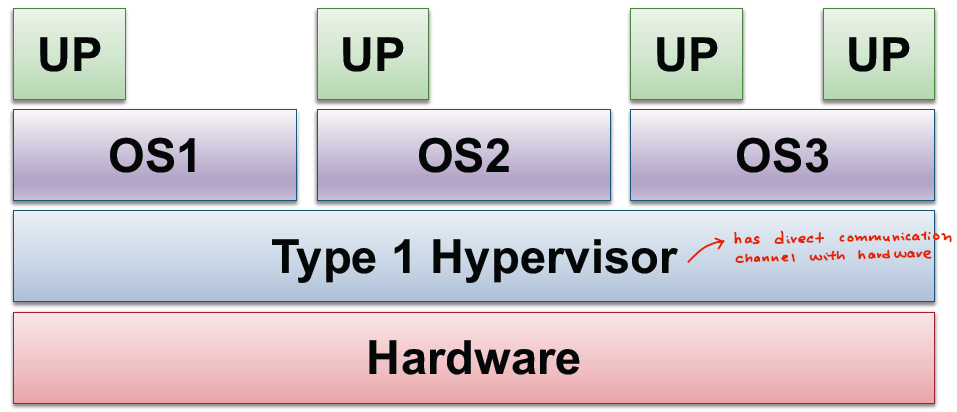
\includegraphics[width=0.39\textwidth]{type_1}%
            \qquad%
            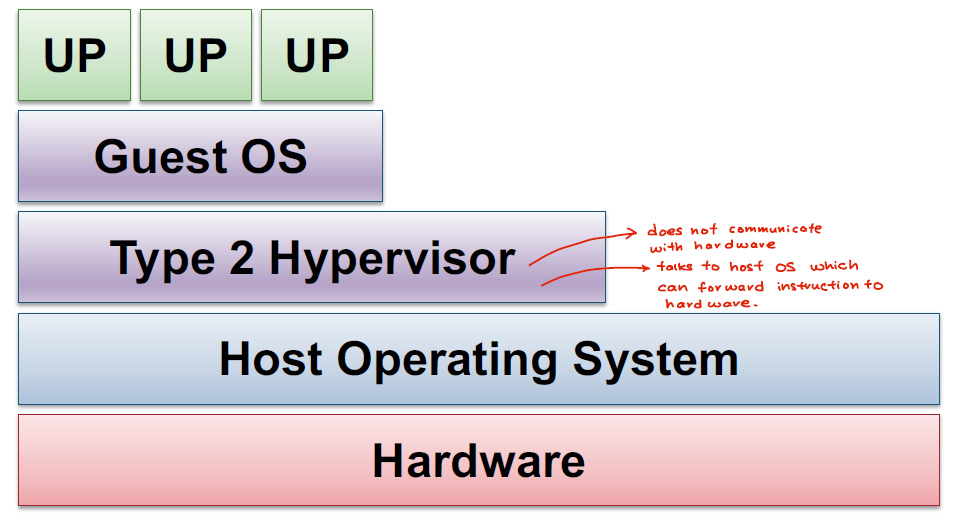
\includegraphics[width=0.39\textwidth]{type_2}%
        \end{minipage}
        \begin{center}
            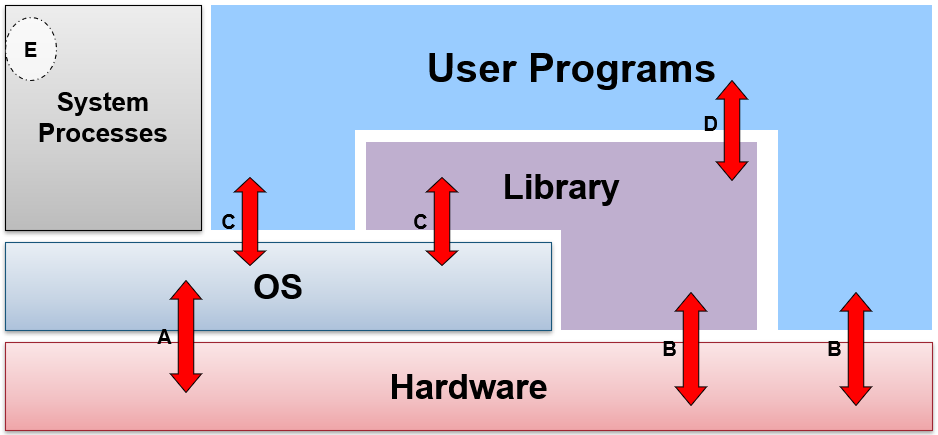
\includegraphics[width=0.35\columnwidth]{interactions}
        \end{center}
        \section{Process Abstraction}
        \subsection{Process Abstraction}
        \begin{itemize}
            \item \textbf{Process}: a dynamic abstraction for executing program
            \item Includes all information required to describe a running program (Memory context, hardware context, OS context)
            \item Information is used to \textbf{context switch} between running programs (to switch from program A to B, we save all information regarding program A then load information of program B)
            \item An executable binary consists of two major components: instructions and data
            \item During execution, more information:
            \begin{itemize}
                \item \textbf{Memory context}: text, data, stack, heap
                \item \textbf{Hardware context}: General Purpose Registers, Program Counter, Stack Pointer, Stack FP, ...
                \item \textbf{OS context}: PID, Process state, Resources used, File Descriptor
            \end{itemize}
        \end{itemize}
        \begin{tabular}{l}
            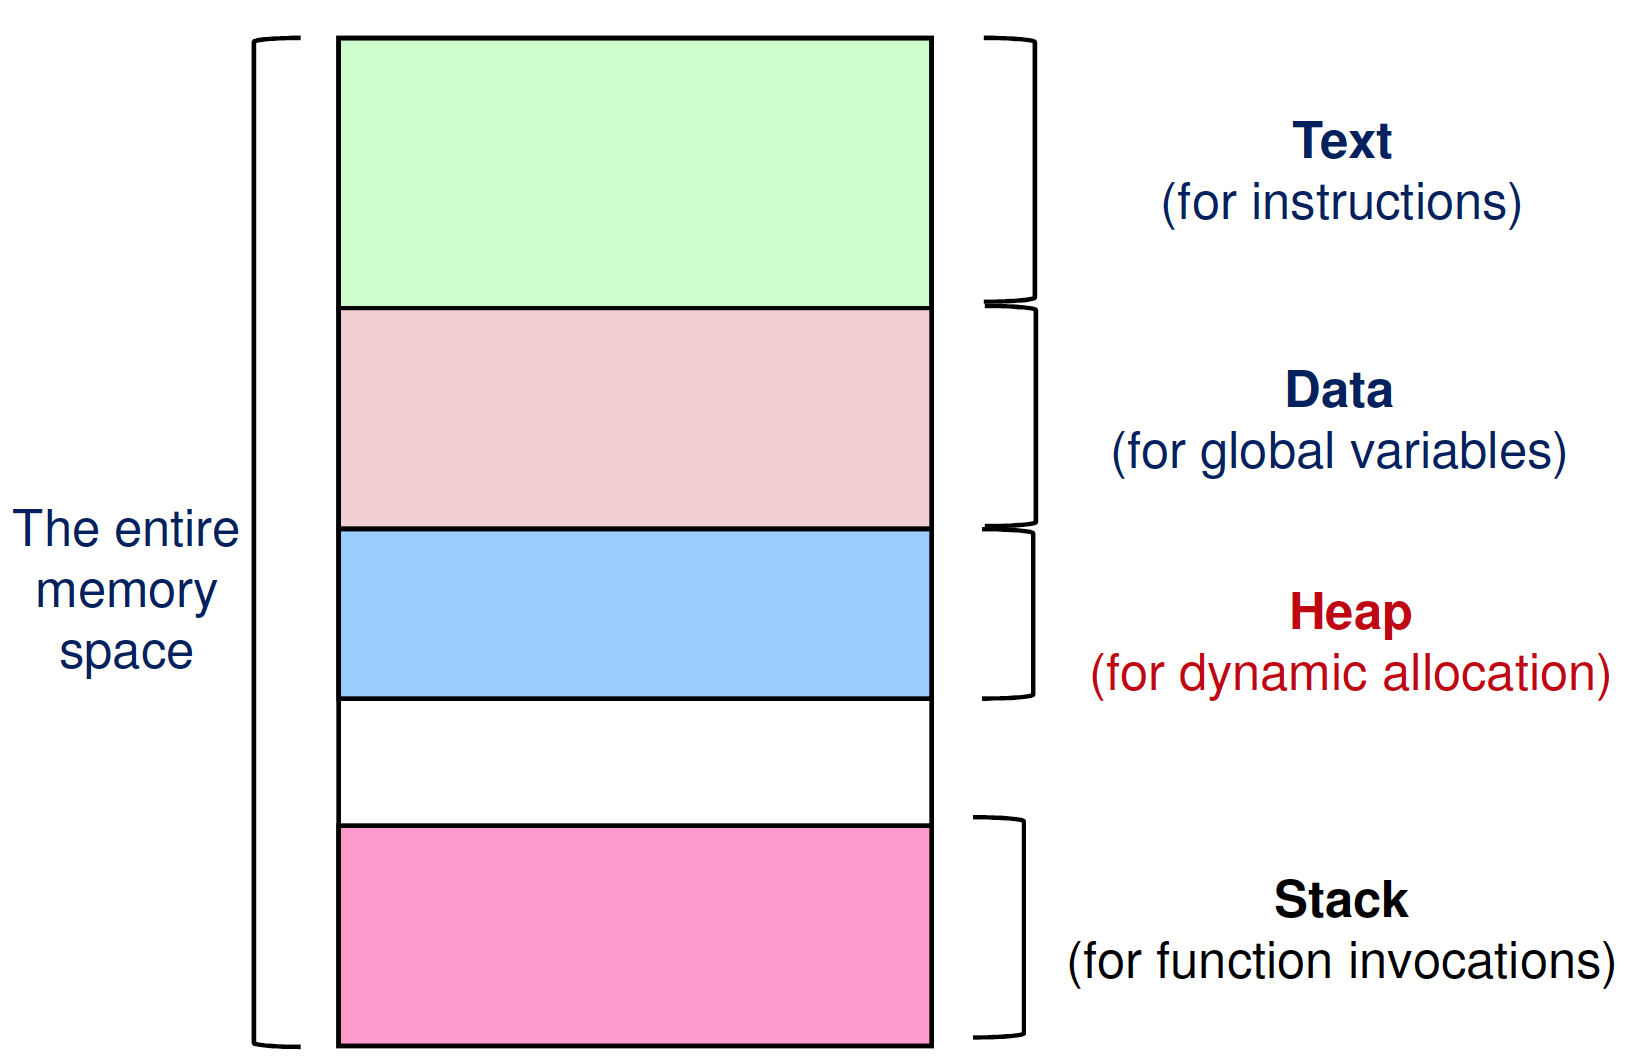
\includegraphics[width=0.5\linewidth]{stack-memory}
        \end{tabular}
        \begin{tabularx}{0.45\columnwidth}{X}
            Note: stack grow upwards in this case
        \end{tabularx}
        \subsection{Memory Hierarchy}
        \begin{center}
            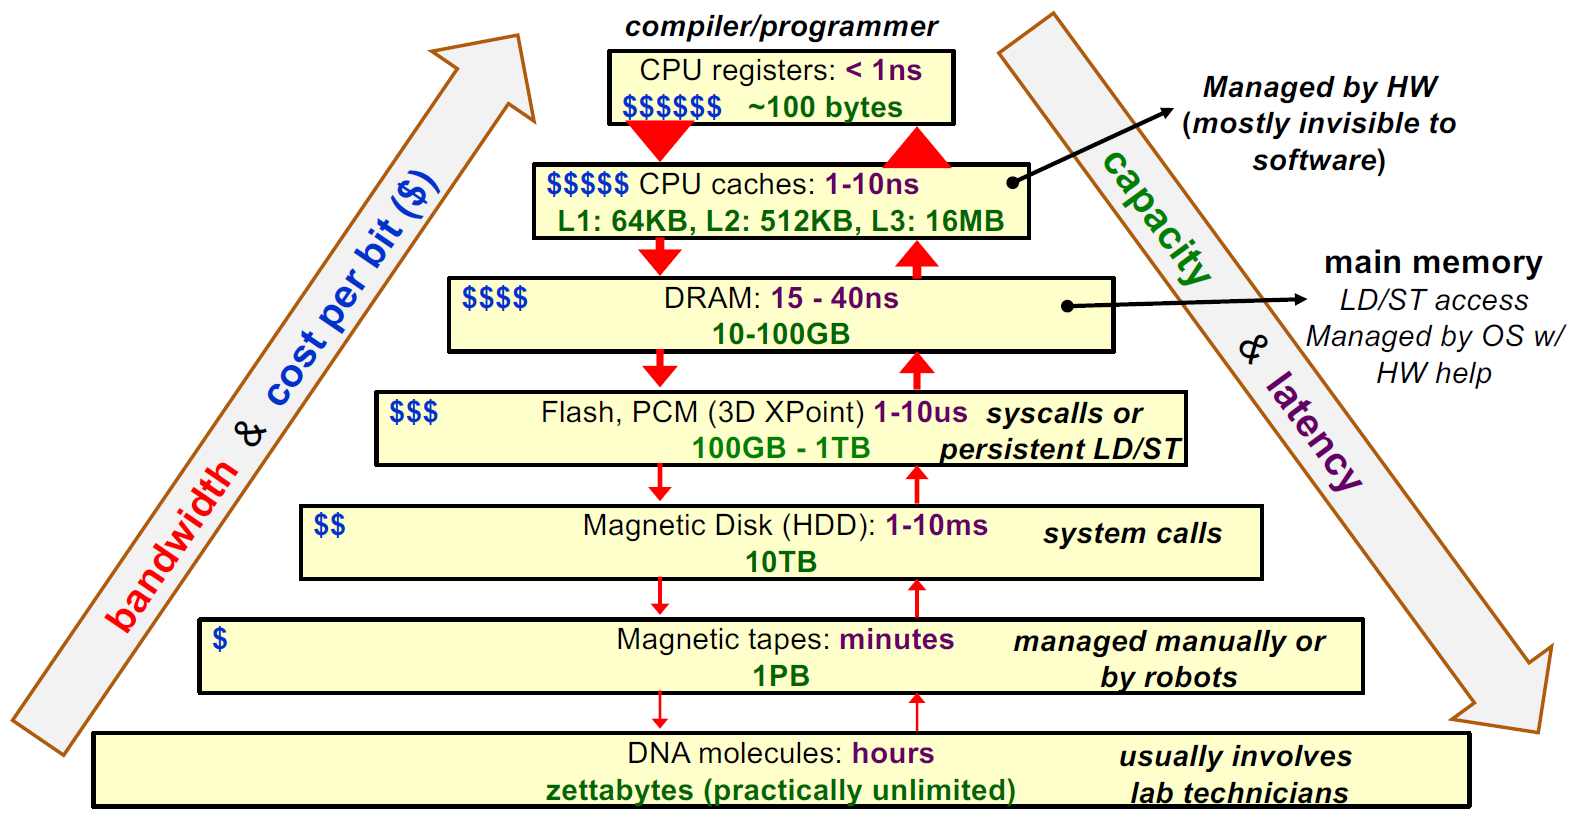
\includegraphics[scale=0.17]{memory_hierarchy}
        \end{center}
        \subsubsection{Caches}
        Caches duplicate part of the memory for faster access (hardware optimization), are fast and invisible to software, usually split into instruction and data cache (optimized differently)
        \subsection{Function calls}
        \subsubsection{Challenges faced when calling functions}
        \begin{itemize}
            \item How to differentiate between global variables and local variables?
            \item Once we return from a function where do we return to? There is no static point of return from a function.
        \end{itemize}
        \subsubsection{Control Flow and Data}
        Important steps (and their corresponding issues):
        \begin{enumerate}
            \item Setup the parameters (Setup "per-function data")
            \item Transfer control to callee (Need some way to jump to function)
            \item Setup local variables (How do we store this so there is no conflict?)
            \item Store result if applicable (Need some way to capture return result)
            \item Return to caller (How do we know where to return to?)
        \end{enumerate}
        \subsection{Stack Memory (LIFO data structure)}
        \begin{itemize}
            \item New memory region to store information of a function invocation
            \item Described by a \textbf{stack frame}, containing: Return address of the caller (PC, old SP), Arguments for the function, Storage for local variables, Frame Pointer, Saved Registers
            \item \textbf{Stack Pointer} = The top of stack region (first unused location)
            \item \textbf{Frame Pointer} = points to a \textbf{fixed location in a stack frame} (platform dependent)
            \item \textbf{Saved Registers} = memory to temporarily hold General Purpose Registers (GPR) value during \textbf{register spilling}* since number of registers are very limited
        \end{itemize}
        * Register spilling occurs when GPRs are exhausted and have to be temporarily be stored on memory so they can be reused
        \subsubsection{Function Call Convention}
        Setup and teardown of the stack frame is usually \textcolor{red}{done by the programmer or the compiler} (we usually don't want the OS to touch the stack)\\\\
        \textbf{Stack Frame Setup}:
        \begin{itemize}
            \item \textbf{Caller}: Pass parameters with registers and/or stack, Save Return PC on stack
            \item \textbf{Callee}: Save the old FP, SP, and registers used by callee, Allocate space for local vars on stack, adjust SP to point to new stack top\\
        \end{itemize}
        \textbf{Stack Frame Teardown}:
        \begin{itemize}
            \item \textbf{Callee}: Place return result on stack, Restore saved registers, FP, SP
            \item \textbf{Caller}: Utilize return result, Continues execution
        \end{itemize}
        \subsection{Dynamically Allocated Memory}
        Using a separate \textbf{heap memory region} that allows for memory space to be acquired during execution time. \textbf{Grows in opposite direction from stack}: to allow for more flexibility since there are times we need more stack memory (e.g. recursion) and sometimes we need more heap memory
        \subsubsection{Behaviour of heap}
        \begin{enumerate}
            \item Allocated only at runtime: size not known during compilation time $\rightarrow$ cannot be placed in Data region
            \item No definite deallocation timing: can be explicitly freed by programmer or implicitly freed by garbage collector $\rightarrow$ cannot be placed on stack
            \item Tends to create "holes" or "fragments" in memory since any portion of the heap can be deallocated at any time $\rightarrow$ need to run defragment programs to compact the heap
        \end{enumerate}
        \subsection{Process Identification \& Process State}
        \begin{itemize}
            \item Using process ID \textbf{(PID)}, a unique number among the processes.
            \item OS dependent issues: Are PID's reused? Are there reserved PID's? Does it limit max number of processes?
        \end{itemize}
        \begin{center}
            \textbf{5 State Process Model}:\\
            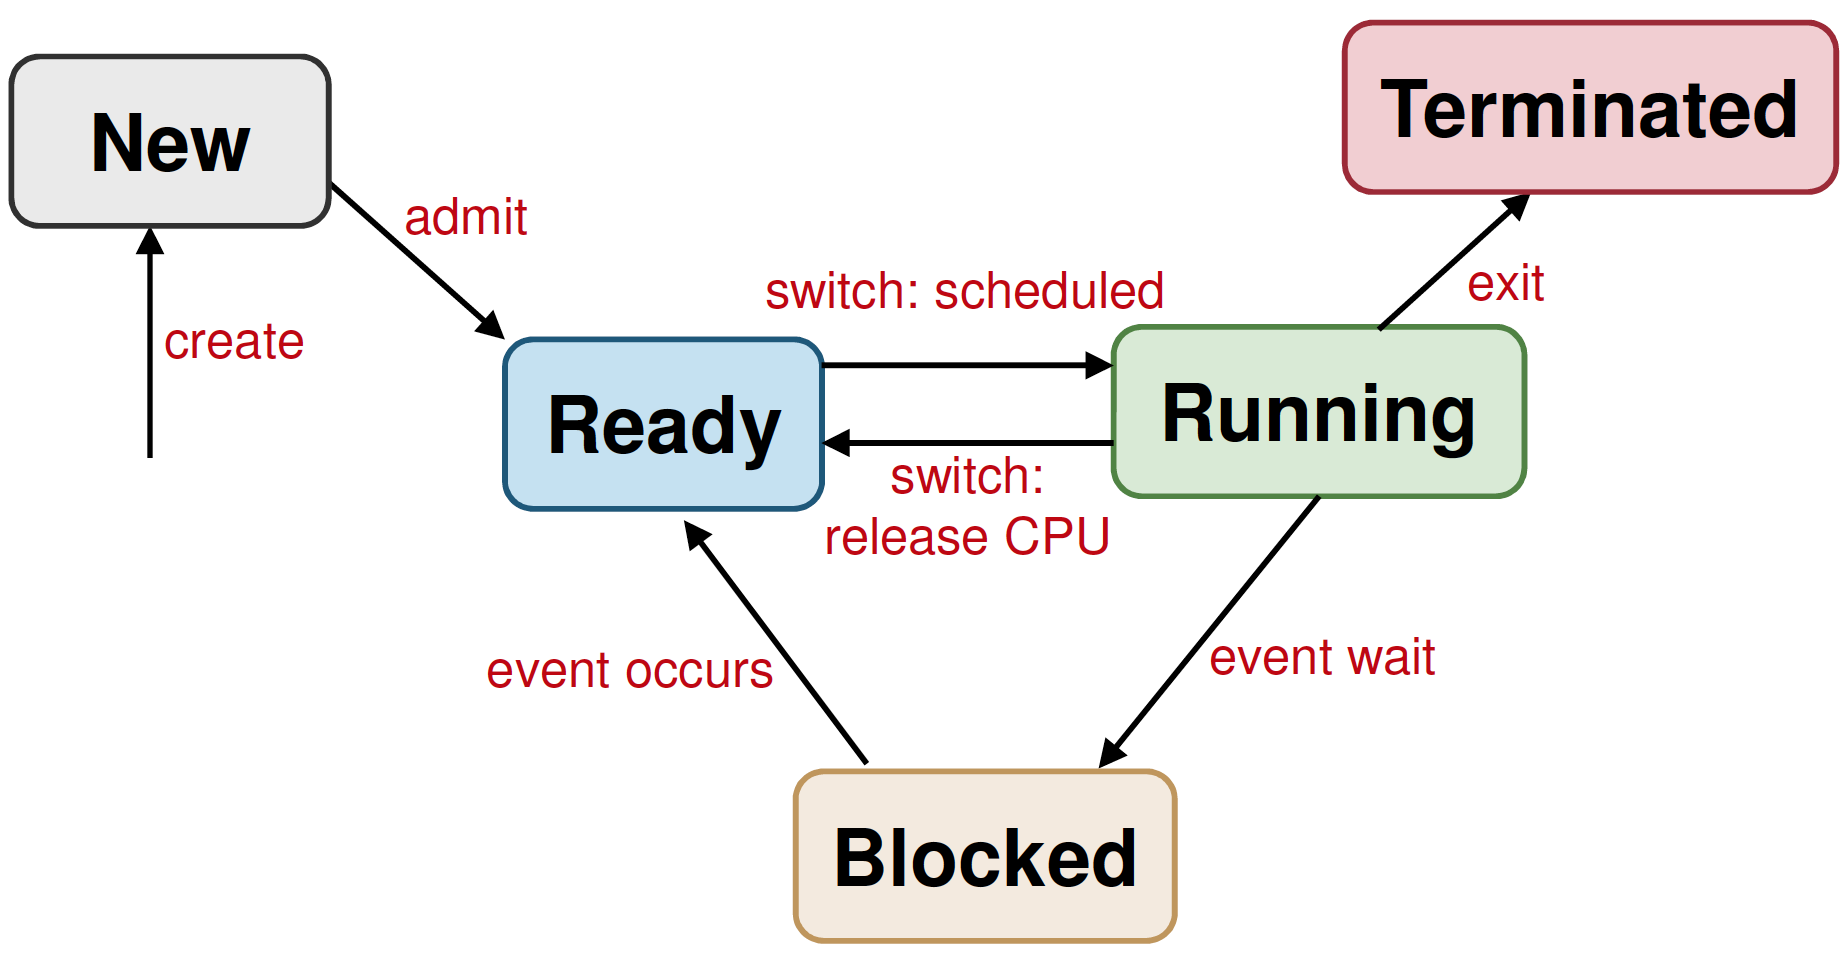
\includegraphics[width=0.7\linewidth]{process-state}
        \end{center}
        \begin{enumerate}
            \item \textbf{New}: process created, may still be initialising, not yet ready
            \item \textbf{Ready}: process is admitted by scheduler waiting to run
            \item \textbf{Running}: process being executed on CPU
            \item \textbf{Blocked}: process waiting, can't execute till event is available
            \item \textbf{Terminated}: process finished execution, may require OS cleanup
        \end{enumerate}
        \textbf{Transitions}:
        \begin{itemize}
            \item nil -> New (Create)
            \item New -> Ready (Admit): Process ready to be scheduled
            \item Ready -> Running (Switch): Process selected to run
            \item Running -> Ready (Switch): Process gives up CPU voluntarily or preempted by scheduler
            \item Running -> Blocked (Event wait): e.g. syscall, waiting for I/O, ...
            \item Blocked -> Ready (Event occurs)
        \end{itemize}
        \textbf{With 1 CPU}:
        \begin{itemize}
            \item $\leq$ 1 process in running state
            \item conceptually 1 transition at a time
        \end{itemize}
        \textbf{With m CPUs}:
        \begin{itemize}
            \item $\leq$ m processes in running state
            \item possibly parallel transitions
            \item each process may be in different states
        \end{itemize}
        \subsection{Process Table \& Process Control Block}
        \begin{tabularx}{0.42\columnwidth}{X}
            \begin{itemize}
                \item \textbf{PCB/Process Table Entry} = entire execution context for a process
                \item \textbf{Process Table} =  kernel maintains PCB for all processes, stored as one table
                \item Stores a bunch of pointers that points to the correct places so that processes can be restored after context switch
                \item Issues: Scalability, Efficiency
            \end{itemize}
        \end{tabularx}
        \begin{tabular}{l}
            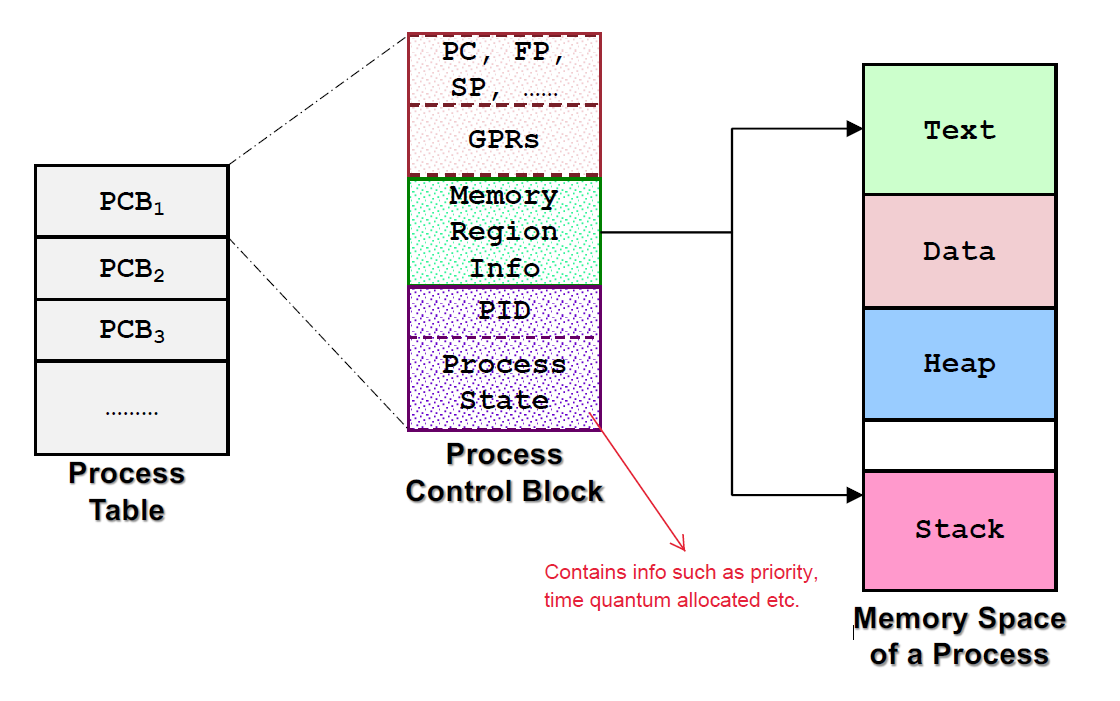
\includegraphics[width=0.55\linewidth]{process-table}
        \end{tabular}
        \subsection{System Calls}
        API to OS -- provides a way of calling services in kernel, different from normal function call in that have to change from user mode -> kernel mode, more expensive due to OS overhead
        \subsubsection{APIs in different OS}
        \begin{itemize}
            \item Unix variants mostly follows POSIX (portable operating interface) standards and typically have a small number of system calls: ~100
            \item Windows uses Win API which typically have a huge number of system calls: ~1000, and new system calls comes with each new version
        \end{itemize}
        \subsubsection{C/C++ Sys calls}
        A C/C++ program can call the library version of system calls. A function wrapper has same name and parameters as the syscall. Alternatively, there is also a function adapter which is user-friendlier (less params, more flexible params value).
        \vfill\null
        \subsubsection{Sys Call Mechanism}
        \begin{enumerate}
            \item User program invokes the library call (normal function call mechanism)
            \item Library call places the system call number in a register
            \item Library call executes \texttt{TRAP} to switch from user mode to kernel mode
            \item In kernel mode, syscall handler is determined using the syscall number as index by \textbf{dispatcher}
            \item System call handler is executed
            \item System call handler ended, control return to library call, switch kernel -> user mode
            \item Library call return to user program via normal function return mechanism
        \end{enumerate}
        * syscall handlers are ptr to functions and are stored in a table to provide efficient lookup
        \subsection{Exception \& Interrupt}
        \textbf{Exception}:
        \begin{itemize}
            \item \textbf{Synchronous}, occurring due to program execution
            \item Effect: have to execute an \textbf{exception handler}, similar to a forced function call
            \item Can explicitly call \texttt{TRAP} to purposely throw exception $\rightarrow$ typically used for debugging
            \item e.g. Overflow, underflow, Divide by 0, Illegal mem address
        \end{itemize}
        \textbf{Interrupt}:
        \begin{itemize}
            \item External events interrupting execution, usually hardware-related (timer, mouse moved, keyboard pressed)
            \item \textbf{Asynchronous}, occurring independent of program execution
            \item Effect: execution is suspended, have to execute \textbf{interrupt handler}
            \item Note that if a program is in the middle of executing an instruction, it would complete that instruction first before passing control to interrupt
            \item Interrupts can be stacked (timer interrupt can take over a mouse interrupt)
        \end{itemize}
        \subsubsection{Handler Routine}
        \begin{enumerate}
            \item Save register/CPU state
            \item Perform handler routine
            \item Restore register/CPU
            \item Return from interrupt
        \end{enumerate}
        * Exception uses software for handler routine whereas interrupts uses hardware\\
        * Handler uses a different hardware context than user programs
        \section{Process Abstraction: Unix}
        \subsection{Process in UNIX}
        Contains information on PID, Process state (running, sleeping, stopped, zombie), Parent PID (PPID), Cumulative CPU time etc.
        \subsection{Process Creation: Fork}
        Fork creates a new process known as \textbf{child process} which is a duplicate of the current executable image (same code, same address space, same PC etc.). \textcolor{red}{Data is a copy of the parent }(i.e. not shared). Only differs in PID, PPID and \texttt{fork()} return value (0 for child and > 0 for parent).
        \subsection{Common UNIX syscalls}
        \begin{itemize}
            \item \mintinline{C}{int execl(char *path, char *arg0, ..., char *argN, NULL);} replaces current executing process image, \textcolor{red}{does not return unless error}. Will not exit on error. Only replaces Code and does not replace PID and other information
            \item \mintinline{C}{void exit(int status);} \texttt{Status} is returned to parent process and has value 0 to represent normal termination, else problematic. Does not return.
            \item \mintinline{C}{int wait(int *status);} returns the PID of terminated child (\textcolor{red}{does not wait for grandchildren}), status stores exit status. Blocking (\textcolor{red}{does not block when process has no children}). Cleans up remainder of child system resources. Note that \textcolor{red}{\texttt{wait()} waits for child even if child calls \texttt{execl()}}
        \end{itemize}
        \subsection{Master Process}
        The common ancestor of all processes is \texttt{init} which is created in kernel at boot up time and has a PID = 1
        \subsection{Process Termination}
        Most system resources used by process are released on exit. Only PID, status and CPU time are not released (to facilitate clean up by parent when it calls \texttt{wait}). Generally, PCB is also not removed. On program termination, open files are flushed automatically.\\\\
        \textbf{Zombie process}: child process terminates but parent did not call \texttt{wait} -- child becomes zombie, can fill up processs table, created so that \texttt{wait()} system call can work properly, user command running in the background is considered a zombie\\
        \textbf{Orphaned Process}: parent terminates before child -- \texttt{init} becomes pseudo-parent, who will call \texttt{wait} on children
        \subsection{Implementing \texttt{\textbf{fork()}}}
        Simplified implementation:
        \begin{enumerate}
            \item Create address space of child process
            \item Allocate p' = \texttt{new PID}
            \item Create entry in Process Table
            \item Copy kernel environment of parent process (e.g. priority for process scheduling)
            \item Initialize child process context: \texttt{PID} = p', \texttt{PPID} = parent ID, \textcolor{red}{zero CPU time}
            \item Copy memory regions, program, stack, data (further optimized by using copy-on-write)
            \item Acquires shared resources (files, current working directory)
            \item Initialize hardware context (Copy registers from parent)
            \item Add child process to scheduler queue
        \end{enumerate}
        * \textbf{Copy-on-write} only duplicates a memory location when it is written to (either by parent or child). When data is read only, memory is shared between parent and child
        \section{Process Scheduling}
        3 categories of \textbf{processing environment}: (1) \textbf{Batch Processing}: no user, no interaction, no need to be responsive, (2) \textbf{Interactive}: with active user interacting, need to be responsive, consistent in response time, (3) \textbf{Real-time Processing}: deadline to meet, usually periodic process
        \subsection{Criteria for Scheduling Algorithms}
        \begin{itemize}
            \item \textbf{Fairness}: fair share of CPU time, no starvation (prevalent in priorty based scheduling)
            \item \textbf{Balanceed}: all parts of the computing system should be utilised (shouldn't have a scenario where all processes are waiting on CPU or I/O)
        \end{itemize}
        \subsection{Types of scheduling policies}
        \begin{itemize}
            \item \textbf{Non-preemptive (cooperative)} -- a process stays scheduled until it blocks/gives up the CPU voluntarily
            \item \textbf{Preemptive}: CPU can be taken from running process at \textcolor{red}{ANY} time. A process is given a fixed time quota to run (possible to block or yield early), at the end of the time quota, the running process is suspended and another process gets picked.
        \end{itemize}
        \subsection{Scheduling a process}
        \begin{enumerate}
            \item Scheduler is triggered (OS takes over)
            \item If context switch is needed: context of current running process is saved, placed on blocked/ready queue
            \item Pick a suitable process \textbf{P} to run based on scheduling algorithm
            \item Setup the context for \textbf{P}
            \item Let process \textbf{P} run
        \end{enumerate}
        \subsection{Scheduling for Batch Processing}
        Criteria:
        \begin{itemize}
            \item \textbf{Turnaround time}: Total time taken (time when it end - time when it arrived), related to waiting time, waiting time = Turnaround time - Time spent doing work (CPU + I/O)
            \item \textbf{Throughput}: Rate of task completion
            \item \textbf{CPU Utilisation}: \% of time when CPU is working on a task, higher the better
        \end{itemize}
        \subsubsection{First-Come First-Served (FCFS)}
        \begin{itemize}
            \item Tasks are stored on a FIFO queue based on arrival time. Pick the head of queue to run until task is done OR task is blocked. Blocked task removed from queue, when it is ready again, placed at back of queue like a newly arrived task.
            \item \textbf{Guaranteed} to have no starvation: \# of tasks in front of task X in FIFO is always decreasing -> task X will get its chance eventually.
            \item Shortcoming: \textbf{Convoy Effect} -- due to non-preemptiveness, one slow process (CPU intensive) slows down the performance of the entire set of processes.
        \end{itemize}
        \subsubsection{Shortest Job First (SJF)}
        \begin{itemize}
            \item Select the task that needs the shortest amount of CPU time, thus \textbf{guarantees} smallest average waiting time (in turn decreasing average turnaround time).
            \item \textbf{Shortcomings}: Need to know total CPU time for a task in advance (have to guess if not available), starvation is possible (biased towards short jobs, long jobs may never run)
            \item Predicting CPU Time, common approach (\textbf{Exponential Average}):\\
            \textcolor{red}{$\text{Predicted}_{n+1} = \alpha \text{Actual}_n + (1-\alpha)\text{Predicted}_n$}, where $\alpha$ represents the significance of immediate past values, and $(1-\alpha)$ represents the significance of past history (typical $\alpha$ value is 1/2)
            \item Higher $\alpha$ cause predicted value to fluctuate closer to the last value, while lower $\alpha$ allow a predicted value that is closer to the historical value
        \end{itemize}
        \subsubsection{Shortest Remaining Time (SRT)}
        \begin{itemize}
            \item Select job with shortest remaining (or expected) time.
            \item Variation of SJF that is \textbf{preemptive} and uses remaining time.
            \item New job with shorter remaining time can preempt currently running job
            \item Provide good service for short jobs even when they arrive late
        \end{itemize}

        \subsection{Scheduling for Interactive Systems}
        \begin{itemize}
            \item
            Criteria:
            \begin{itemize}
                \item \textbf{Response time}: Time between request and response by system (time when it first start running - time when it first reach)
                \item \textbf{Predictability}: Lesser variation in response time $\rightarrow$ better predictability
            \end{itemize}
            \item \textbf{Preemptive} scheduling algorithms are used to ensure good response time, thus scheduler needs to run periodically.
            \item \textbf{Timer interrupt} = interrupt that goes off periodically based on hardware clock, OS ensures timer interrupt is not intercepted by other program/interrupt
            \item Timer interrupt handler \textbf{invokes OS scheduler}.
            \item \textbf{Interval of Timer Interrupt (ITI)} typically 1-10ms, scheduler is triggered every ITI but may not actually run
            \item \textbf{Time Quantum} = execution duration given to a process, can be constant/variable, must be multiple of ITI (commonly 5-100ms)
        \end{itemize}
        \subsubsection{Round Robin (RR)}
        \begin{itemize}
            \item Tasks stored in a FIFO queue, pick task from head of queue until time quantum elapsed OR task gives up CPU voluntarily OR task blocks
            \item Basically a \textbf{preemptive version of FCFS}
            \item \textbf{Response time guarantee}: given $n$ tasks and quantum $q$, time before a task get CPU is bounded by $(n-1)q$, note that \textcolor{red}{bounded response time $\neq$ responsive}
            \item Choice of time quantum: big = better CPU utilization, longer waiting time; small = bigger overhead (worse CPU utilization) but shorter waiting time
        \end{itemize}
        \subsubsection{Priority Scheduling}
        \begin{itemize}
            \item Assign a \textbf{priority} value to all tasks, select task with highest priority value.
            \item \textbf{Preemptive}: higher priority process can preempt running process with lower priority
            \item \textbf{Non-preemptive}: late coming high priority process has to wait for next round of scheduling
            \item \textbf{Shortcomings}: Low priority process \textbf{can starve}, worse in preemptive variant
            \item \textbf{Possible solutions}: Decrease the prioty of currently running process after every time quantum, Give each process a minimum time quantum
            \item Generally hard to guarantee/control exact amount of CPU time given to a process
            \item \textbf{Priority Inversion}: 3 processes, priorities Hi, Mi, Lo. L locks resource, M pre-empts L, A arrives and tries to lock same resource as L. Then M continues executing although H has higher priority.
        \end{itemize}
        \subsubsection{Multi-level Feedback Queue (MLFQ)}
        \begin{itemize}
            \item Designed to solve the issue of scheduling without perfect knowledge (e.g. no need to guess and estimate running time)
            \item Adaptive, minimising both response time for IO-bound and turnaround time for CPU-bound
            \item Rules:
            \begin{itemize}
                \item Priority(A) $>$ Priority(B) -> A runs (\textcolor{red}{after B time quantum is up})
                \item Priority(A) == Priority(B) -> A and B runs in RR
                \item New job -> highest priority
                \item If a job fully utilised its time slice -> priority reduced
                \item If a job gives up/blocks before it finishes the time slice -> priority retained
            \end{itemize}
            \item \textbf{Shortcomings}: (1) \textbf{Starvation} -- if there are too many interactive jobs, long-running jobs will starve, (2) gaming the scheduler by running for 99\% of time quantum, then relinquish the CPU (\textbf{hogging CPU}), (3) a program may change its behaviour CPU-bound -> interactive (\textbf{not given priority when it is needed})
            \item Possible solution:
            \begin{itemize}
                \item \textbf{Priority boost}: Periodically move all processes to highest priority. \textcolor{red}{guaranteeing no starvation }as highest priority -> RR, also allows processes with different behaviour phases to be treated correctly even after it reach lowest priority
                \item \textbf{Cumulative Time Quantum}: Once a job uses up its time allotment at a given level, its priority is reduced
            \end{itemize}
        \end{itemize}
        \subsubsection{Lottery Scheduling}
        \begin{itemize}
            \item Give out "lottery tickets" to processes. When a scheduling decision is needed, a ticket is chosen randomly among eligible tickets.
            \item In the long run, a process holding X\% of tickets can win X\% of the lottery held and use the resource X\% of the time.
            \item \textbf{Responsive}: newly created process can participate in next lottery, every process gets to run in every round (\textcolor{red}{waiting time is bounded by $2\times{N}\times{}$TQ})
            \item Good level of control: A process can be given lottery tickets to be distributed to its child process, an important process can be given more lottery tickets, each resource can have its own set of tickets
            \item Simple implementation
        \end{itemize}

        \section{Inter-Process Communication}
        \begin{itemize}
            \item 2 common IPC mechanisms: \textbf{Shared-Memory} \& \textbf{Message Passing}
            \item 2 Unix-specific IPC mechanisms: \textbf{Pipe} and \textbf{Signal}
        \end{itemize}
        \subsection{Shared-Memory}
        \begin{itemize}
            \item \textcolor{red}{Implicit communication} through reads/writes to shared variables
            \item General idea: Process $p_1$ creates a shared memory region $M$ in \textbf{\textcolor{red}{user space}}, process $p_2$ attaches $m$ to its own memory space. $p_1$ and $p_2$ can now communicate using memory region $M$. Values written to $M$ is visible to all processes that share $M$.
            \item Shared memory region is identified by a number, memory address is only generated when a process attaches to the identified region
            \item Shared memory region can be accessed by any process (set permission bits to \texttt{0666})
            \item OS involved only in creating and attaching shared memory region
            \item \textbf{Advantages}: Efficient (only initial steps involves OS), Ease of use (information of any type or size can be written easily)
            \item \textbf{Disadvantages}: Synchronisation (shared resource -> need to synchronise access), Implementation is usually harder, Limited to a single machine (software abstractions can be supported in distributed systems but less efficient)
            \item In Unix: (1) create/locate shared memory region $M$, (2) Attach $M$ to process memory space, (3) Read/Write $M$, (4) Detach $M$ from memory space after use, (5) Destroy $M$ (only 1 process does this, can only destroy if $M$ is not attached)
        \end{itemize}
        \subsection{Message Passing}
        \begin{itemize}
            \item \textcolor{red}{Explicit communication} through exchange of messages
            \item General idea: process $p_1$ prepares a message $M$ and send it to process $p_2$, $p_2$ receives the message $M$. Sending and receiving messages are generally provided using syscalls (OS mediates it $\rightarrow$ easier to implement, safer but slower since involves OS overhead)
            \item Message has to be stored in \textbf{\textcolor{red}{kernel memory space}}, every send/receive operation is a syscall
            \item \textbf{Advantages}: Portable (can be easily implemented on different processing environment), Easier synchronisation (using synchronous primitive)
            \item \textbf{Disadvantages}: Inefficient (usually requiring OS intervention), Harder to use (message usually limited in size and/or format)
        \end{itemize}
        \subsubsection{Naming \textmd{(how to identify the other party in the comm):}}
        \begin{itemize}
            \item \textbf{Direct Communication}
            \begin{itemize}
                \item Sender/receiver \textbf{explicitly} name the other party (using PID)
                \item Characteristics: 1 link/pair of communicating processes, need to know the identity of the other party
            \end{itemize}
            \item \textbf{Indirect Communication}
            \begin{itemize}
                \item Message are sent to/received (\textcolor{red}{copied}) from message storage (aka mailbox or port)
                \item Characteristic: 1 mailbox can be shared among a number of processes
                \begin{itemize}
                    \item Introduces a problem of who receives the message? There are many variations used: one-to-one, one-to-many, many-to-many, many-to-one
                    \item Since mailbox is in kernel space, OS takes care of synchronisation of message reading and writing
                \end{itemize}
            \end{itemize}
        \end{itemize}
        \begin{center}
            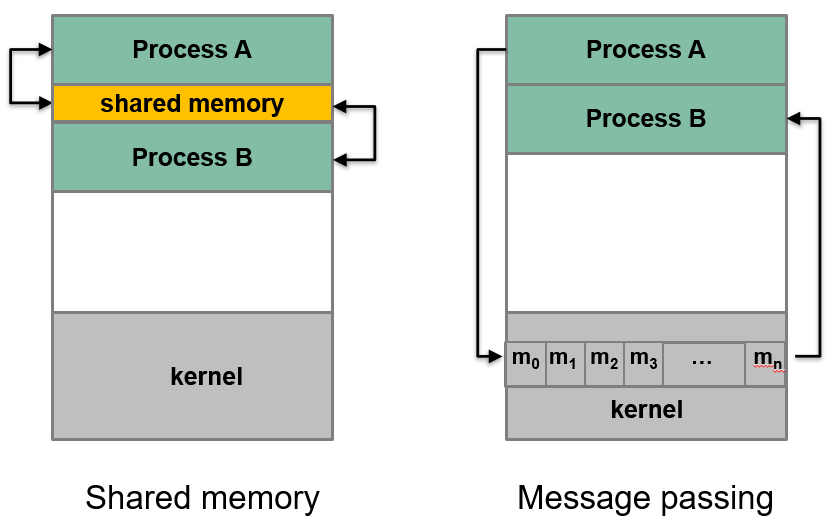
\includegraphics[width=0.57\columnwidth]{shared_vs_passing}
        \end{center}
        \subsubsection{Synchronisation \textmd{(behaviour of the sending/receiving ops)}}
        \begin{itemize}
            \item \textbf{Blocking primitives} (synchronous): sender/receiver is blocked until message is received/has arrived
            \item \textbf{Non-blocking Primitive} (asynchronous): sender resume operation immediately, receiver either receive message if available or proceeds empty handed but doesn't block
            \item Typically \texttt{receive()} is blocking $\rightarrow$ we look at the behaviour of sender to determine whether asynchronous or synchronous
        \end{itemize}
        \subsubsection{Asynchronous Message Passing}
        \begin{itemize}
            \item Assumes that \texttt{receive()} is blocking and sender is non-blocking
            \item System buffers the message (Async message passing \textbf{MUST} have a buffer)
            \item Drawbacks:
            \begin{itemize}
                \item Too much freedom for programmer, program becomes complex
                \item Finite buffer size means system is not truly asynchronous $\rightarrow$ \textcolor{red}{sender waits when buffer is full}
            \end{itemize}
            \item Buffer: Under OS control $\rightarrow$ Synchronization burden placed on OS; Decouples sender and receiver $\rightarrow$  less sensitive to variations in execution $\rightarrow$ don't have to wait on each other unnecessarily.
        \end{itemize}
        \subsubsection{Synchronous Message Passing}
        \begin{itemize}
            \item Assumes sender is blocking and receiver is also blocking
            \item \textbf{No intermediate buffers needed}
            \item \textbf{Pros}:
            \begin{itemize}
                \item Applicable \textbf{beyond single machine}
                \item \textbf{Portable}: Easily implemented on many platforms; Parties on different platforms can communicate
                \item \textbf{Easier synchronization}: Implicit, defined by blocking semantics; No shared memory region (message is copied); Achieves both communication and synchronization simultaneously
            \end{itemize}
            \item \textbf{Cons}:
            \begin{itemize}
                \item \textbf{Inefficient}: Requires OS intervention on every send/receive
                \item \textbf{Harder to use}: Requires packing/unpacking data into supported format
            \end{itemize}
        \end{itemize}
        \subsection{Unix Pipes}
        \begin{itemize}
            \item A communication channel with 2 ends, for reading and writing.
            \item A pipe can be shared between 2 processes (producer-consumer)
            \item Behaviour: like an anonymous file, \textbf{FIFO} (in-order access)
            \item Pipe functions as \textbf{circular bounded byte buffer with implicit synchronisation}: writers wait when buffer full, readers wait when buffer empty (\textbf{Async} sending)
            \item Variants: Multiple readers/writers, half-duplex (unidirectional) or full-duplex (bidirectional)
            \item \mintinline{C}{int pipe(int fd[]);} returns 0 = success. \mintinline{C}{fd[0]} reading end, \mintinline{C}{fd[1]} writing end
        \end{itemize}
        \subsection{Unix Signal}
        \begin{itemize}
            \item An \textbf{async} notification regarding an event sent to a process/thread (OS $\rightarrow$ user program OR user program $\rightarrow$ user program)
            \item Recipient of signal handle by a default set of handlers OR user-supplied handler (only applicable to some signals)
            \item Common signals in Unix: SIGKILL, SIGSTOP, SIGCONT, etc.
        \end{itemize}
        \section{Process Alternative -- Threads}
        \begin{itemize}
            \item Motivation:
            \begin{itemize}
                \item Process is expensive: under \texttt{fork()} model -- duplicate memory space and process context, context switch requires saving/restoration of process information
                \item Hard for independent processes to communicate with each other: independent memory space -- no easy way to pass information, requires Inter-Process Communication (IPC)
            \end{itemize}
            \item A \textbf{traditional process has a single thread of control} -- only one instruction of the whole program is executing at any one time. Instead, we add more threads of control such that multiple parts of the program are executing simultaneously conceptually.
            \item Essential with multi-core architectures
            \begin{itemize}
                \item \textbf{Data parallelism}: different threads doing same task on different data (typically GPU does this)
                \item \textbf{Task parallelism}: different threads do different tasks on same/different data
            \end{itemize}
        \end{itemize}
        \subsection{Process and Thread}
        \begin{itemize}
            \item A single process can have multiple threads
            \item Threads in the same process shares:
            \begin{itemize}
                \item \textbf{Memory Context}: Text, data, heap
                \item \textbf{OS Context} (PID, other resources like files, etc.)
            \end{itemize}
            \item Threads have unique:
            \begin{itemize}
                \item Identification (Thread id)
                \item Registers (general purpose \& special, including PC)
                \item Stack
            \end{itemize}
        \end{itemize}
        \subsubsection{Context Switching}
        \begin{itemize}
            \item \textbf{Process} context switch involves: OS Context, Hardware Context, Memory Context
            \item \textbf{Thread} switch within the same process involves: Hardware context (registers, "stack" -- actually just changing FP and SP)
            \item Can think of threads as a lighter weight process
        \end{itemize}
        \begin{center}
            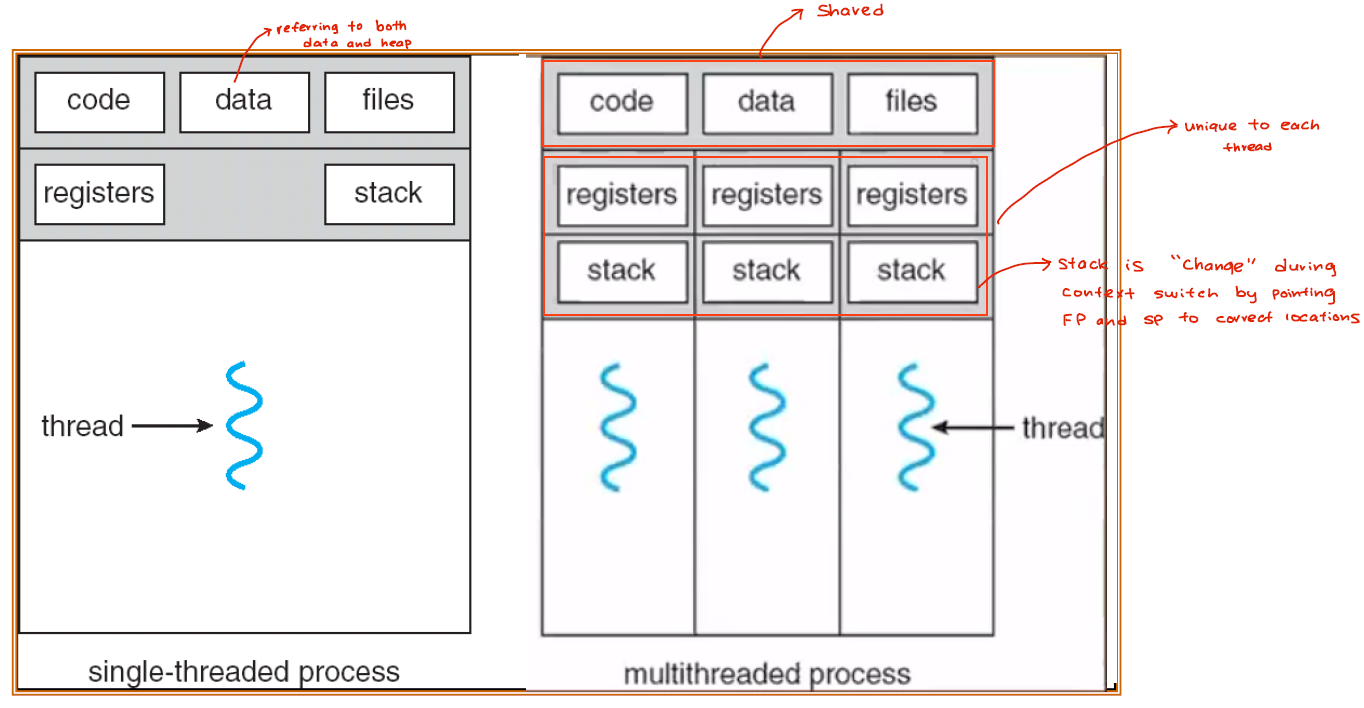
\includegraphics[width=0.65\columnwidth]{thread_illustration}
        \end{center}
        \subsection{Benefits}
        \begin{itemize}
            \item \textbf{Economy}: requires much less resources
            \item \textbf{Resource sharing}: Threads shares most resources, no need for additional information passing mechanism
            \item \textbf{Responsiveness}: multithreaded programs can appear much more responsive (one thread can deal with I/O while another is processing data)
            \item \textbf{Scalability}: Multithreaded program can take advantage of multiple CPUs
        \end{itemize}
        * Note that using threads on a SINGLE CORE does not actually speed up execution time and might instead make it run slower due to overhead
        \subsection{Problems}
        \begin{itemize}
            \item \textbf{Synchronization around shared memory is difficult to handle} -- All memory shared except the stack
            \item \textbf{System call concurrency} -- have to guarantee correctness and determine the correct behaviour of threads ran in parallel
            \item \textbf{Process behaviour} -- impact on process operations, e.g. does \texttt{fork()} duplicate threads? If single thread executes \texttt{exit()}, how abut the whole process? If a single thread calls \texttt{exec()}, how about other threads etc.
        \end{itemize}
        \subsection{Thread Models}
        \begin{itemize}
            \item \textbf{User Thread}
            \begin{itemize}
                \item Implemented as a \textbf{user library}, a runtime system in the process handles thread operations (user or library has to handle multiplexing of threads)
                \item Kernel is \textcolor{red}{not aware} of threads in the process.
                \item \textbf{Advantages}: Multithreaded program on ANY OS (ensures portability and backward compatibility), thread operations are just library calls, more configurable and flexible (such as customised thread scheduling policy)
                \item \textbf{Disadvantages}: OS is not aware of threads, scheduling is performed at \textcolor{red}{process level}. One thread blocked $\rightarrow$ process blocked $\rightarrow$ all threads blocked, cannot exploit multiple CPUs (1 solution is to do Async I/O operation)
            \end{itemize}
            \begin{center}
                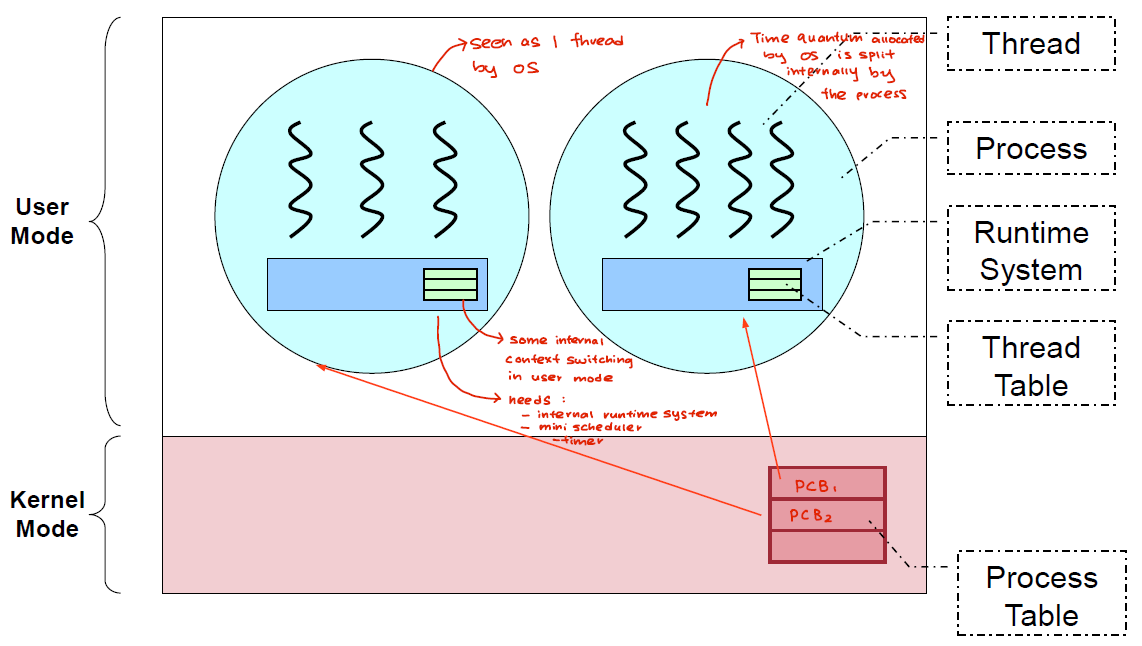
\includegraphics[width=0.65\columnwidth]{user_thread}
            \end{center}
            \item \textbf{Kernel Thread}
            \begin{itemize}
                \item Implemented in the \textbf{OS}, thread operation handled as \textbf{system calls}.
                \item Allows for \textcolor{red}{Thread-level scheduling}, basically treat kernel threads as its own process
                \item Kernel may make use of threads for its own execution
                \item \textbf{Advantages}: Kernel can schedule on thread level (threads on same process can run simultaneously on multiple CPUs $\rightarrow$ 1 thread can be blocked and the rest can still run)
                \item \textbf{Disadvantages}: Thread operation is a syscall (slower and more resource intensive), generally less flexible (used by all multithreaded programs -- many features: expensive, overkill for simple program, few features: not flexible enough for some)
            \end{itemize}
            \begin{center}
                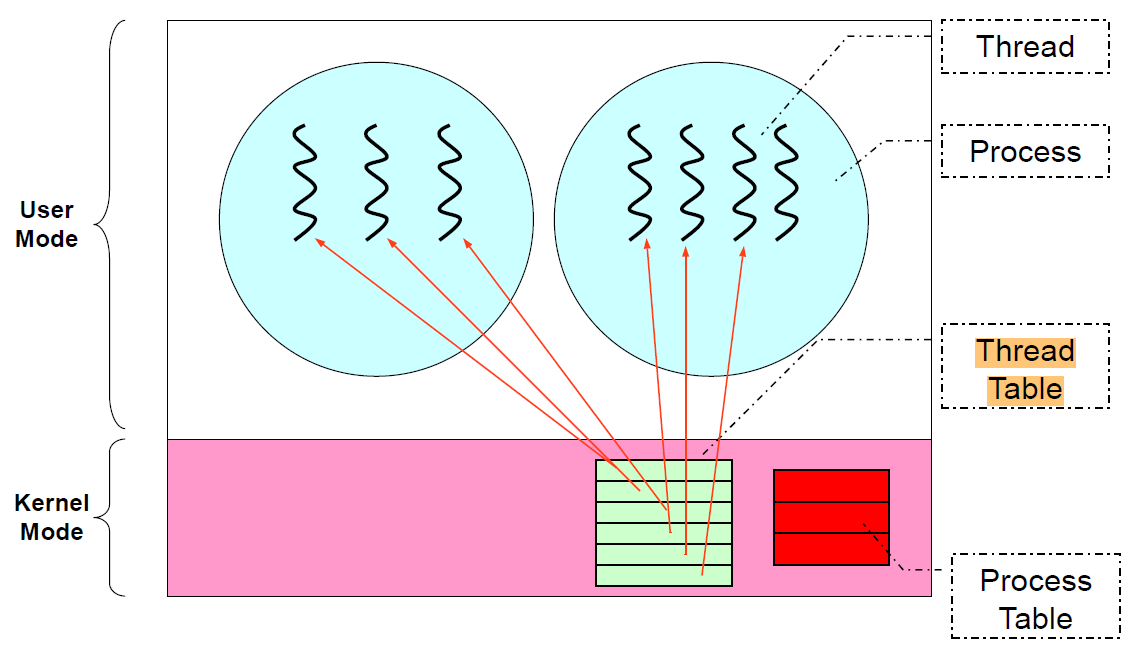
\includegraphics[width=0.65\columnwidth]{kernel_thread}
            \end{center}
            \item \textbf{Hybrid Thread Model}:
            \begin{itemize}
                \item Have \textbf{both kernel and user threads}, OS schedule on kernel threads only, user thread can bind to a kernel thread.
                \item Great flexibility (can limit concurrency of any process/user)
            \end{itemize}
            \begin{center}
                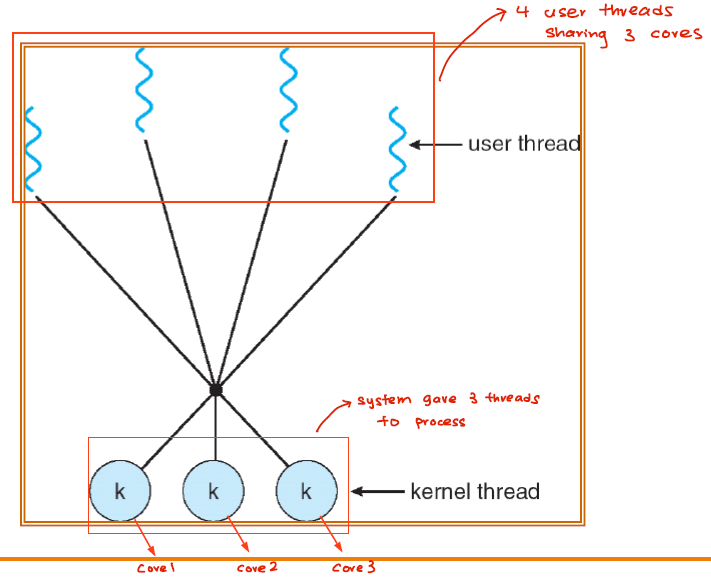
\includegraphics[width=0.7\columnwidth]{hybrid_thread}
            \end{center}
        \end{itemize}
        \subsection{Threads on Modern Processor (Intel Hyperthreading)}
        \begin{itemize}
            \item Threads started off as software mechanism: Userspace lib -> OS aware mechanism
            \item Hardware support on modern processors, supplying multiple sets of registers to \textbf{allow threads to run natively and parallelly on the same core}: \textcolor{red}{Simultaneous Multi-Threading (SMT)}
        \end{itemize}
        \subsection{POSIX Threads: \texttt{pthread}}
        \begin{itemize}
            \item Standard by IEEE, defining API and behaviour.
            \item Implementation is not specified $\rightarrow$ pthread can be implemented as user thread (windows) or kernel thread (Linux)
            \item \mintinline{C}{int pthread_create(pthread_t* tidCreated, const pthread_attr_t* threadAttributes, void* (*startRoutine) (void*), void* argForStartRoutine);}
            \begin{itemize}
                \item \texttt{tidCreated}: Thread ID for the created thread
                \item \texttt{threadAttributes}: Control the behaviour of new thread
                \item \texttt{startRoutine}: Function pointer to the function to be executed by thread
                \item \texttt{argForStartRoutine}: Arguments for the startRoutine function
            \end{itemize}
            \item \mintinline{C}|int pthread_exit(void* exitValue)|
            \begin{itemize}
                \item if \texttt{pthread\_exit()} is not called, a pthread will terminate automatically at the end of startRoutine
                \item if \texttt{"return XYZ"} is used, the "XYZ" is captured as exit value
            \end{itemize}
            \item \mintinline{C}{int pthread_join(pthread_t threadID, void **status);}
            \begin{itemize}
                \item threadID: \texttt{TID} of the pthread to wait for
                \item status: Exit value returned by the pthread
            \end{itemize}
            \item except for \texttt{pthread\_exit}, return 0 = success
        \end{itemize}
        \vfill\null
        \columnbreak
        \section{Synchronization}
        \subsection{Race Condition}
        \begin{itemize}
            \item When 2/more processes \textbf{execute concurrently} in interleaving fashion AND \textbf{share a modifiable resource} resulting in non-deterministic execution.
            \item \textbf{Solution}: designate code segment with race condition as \textbf{critical section} where at any point in time only 1 process can execute. Ideally, process in critical section should be done atomically (you either do it or you don't, cannot be done "halfway")
        \end{itemize}
        \subsection{Critical Section}
        Properties of correct implementation:
        \begin{itemize}
            \item \textbf{Mutual Exclusion}: if a process is executing in critical section, all other processes are prevented from entering it (\textbf{most critical property}, if this fails we disregard the rest)
            \item \textbf{Progress}: If no process is in critical section, one of the waiting processes should be granted access
            \item \textbf{Bounded Wait}: After a process $p_i$ requests to enter the critical section, $\exists$ an upper-bound of number of times other processes can enter the critical section before $p_i$
            \item \textbf{Independence}: process not executing in critical section should never block other processes
        \end{itemize}
        * Note that \textbf{Progress and Independence are related}. Not possible to have progress but no independence but possible to have independence but no progress (Attempt 3)
        \subsubsection{Symptoms of incorrect synchronisation}
        \begin{itemize}
            \item usually due to lack of mutual exclusion
            \item \textbf{Deadlock}: all processes \textcolor{red}{blocked} $\rightarrow$ no progress (e.g. 2 processes using message passing, both processes are using blocking receive and waiting to receive msg from the other). Fulfils the following conditions:
            \begin{enumerate}
                \item \textbf{Mutual Exlusion}: Each resource is either assigned to exactly one process or to none
                \item \textbf{Hold-and-wait}: Processes holding resources can ask for more resources
                \item \textbf{No-preemption}: Cannot forcibly take away resources previously given
                \item \textbf{Circular wait}: Must have a circular list of two or more processes, each waiting for a resource held by the next
            \end{enumerate}
            \item \textbf{Livelock}: processes keep changing state to avoid deadlock and make no other progress, typically \textcolor{red}{processes are not blocked}
            \item \textbf{Starvation}: some processes are blocked forever
        \end{itemize}
        \subsection{Implementations of Critical Section}
        \subsubsection{Incorrect Attempt 1}
        \begin{center}
            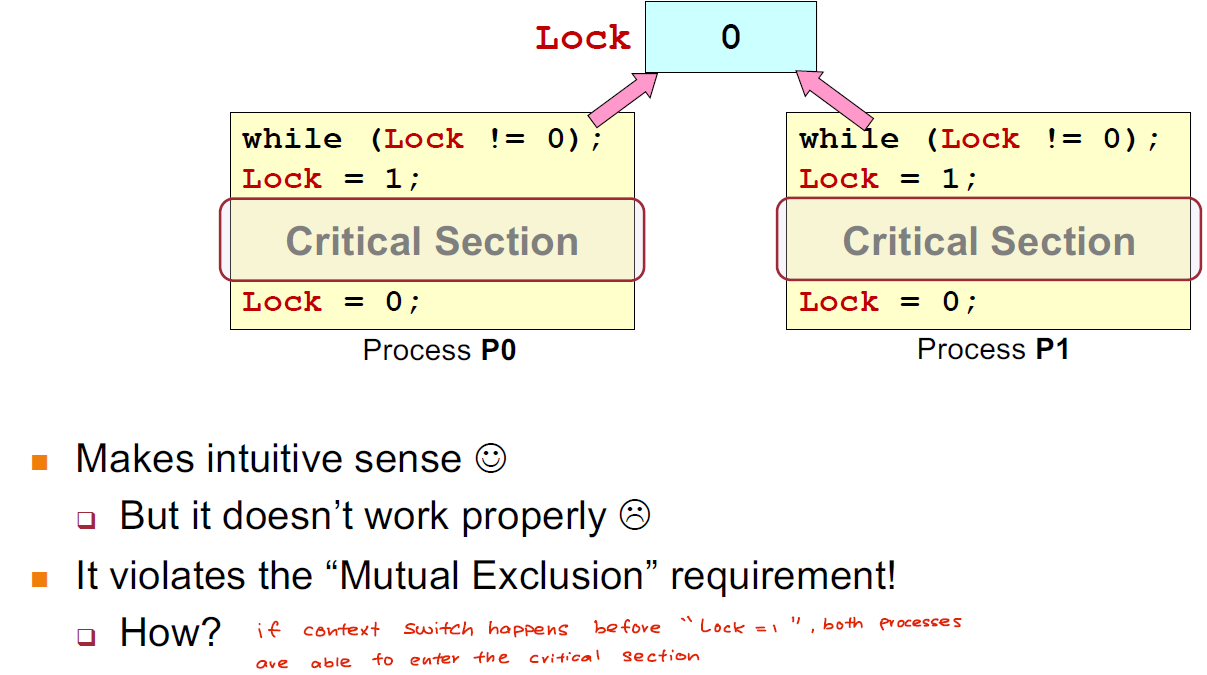
\includegraphics[width=0.9\columnwidth]{attempt_1}
        \end{center}
        \subsubsection{Attempt 1 Incorrect Fix}
        \begin{center}
            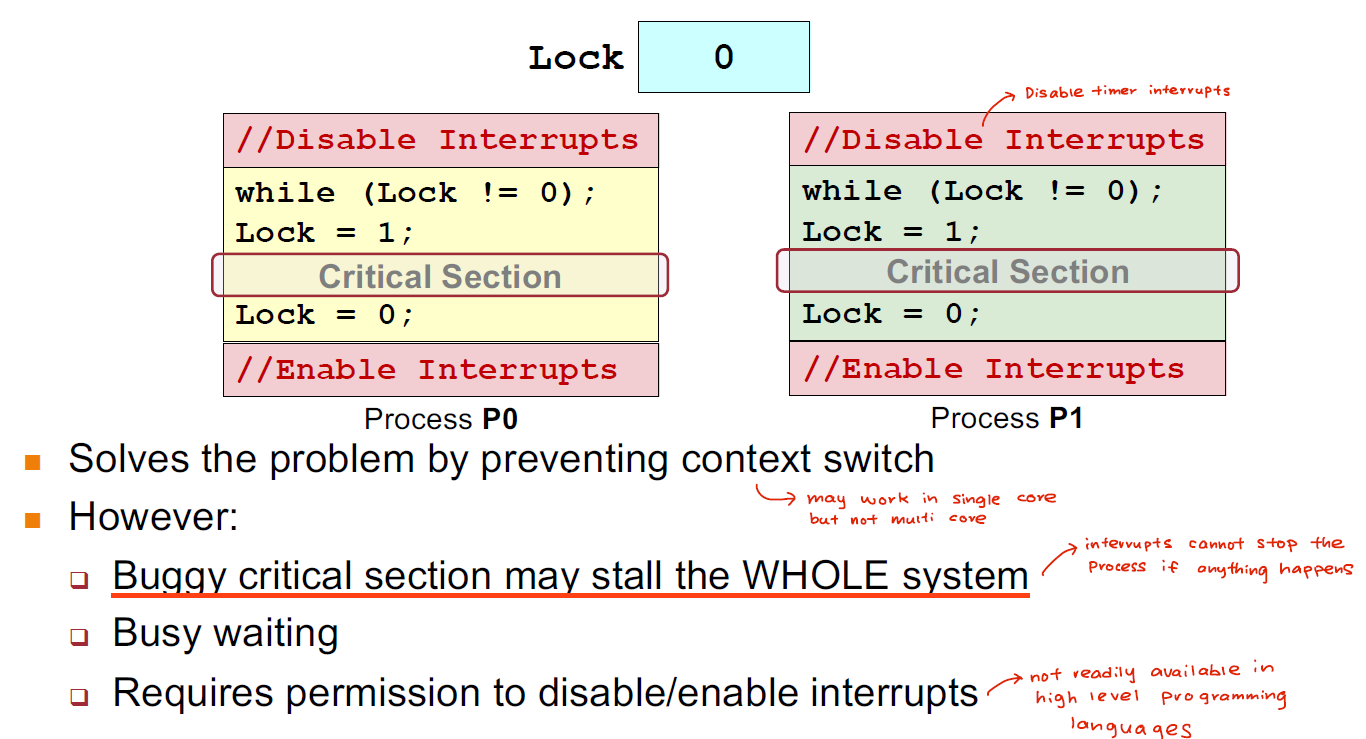
\includegraphics[width=0.9\columnwidth]{attempt_1_fix}
        \end{center}
        \subsubsection{Incorrect Attempt 2}
        \begin{center}
            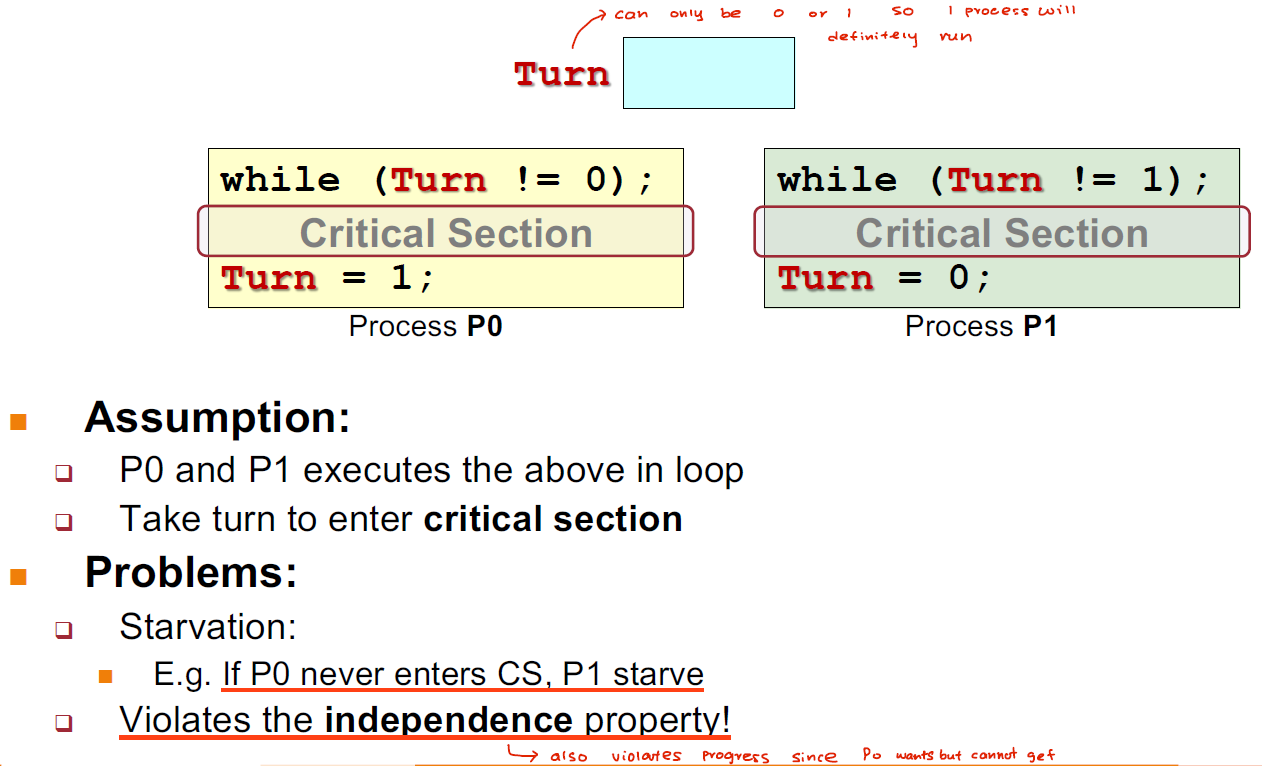
\includegraphics[width=0.9\columnwidth]{attempt_2}
        \end{center}
        \subsubsection{Incorrect Attempt 3}
        \begin{center}
            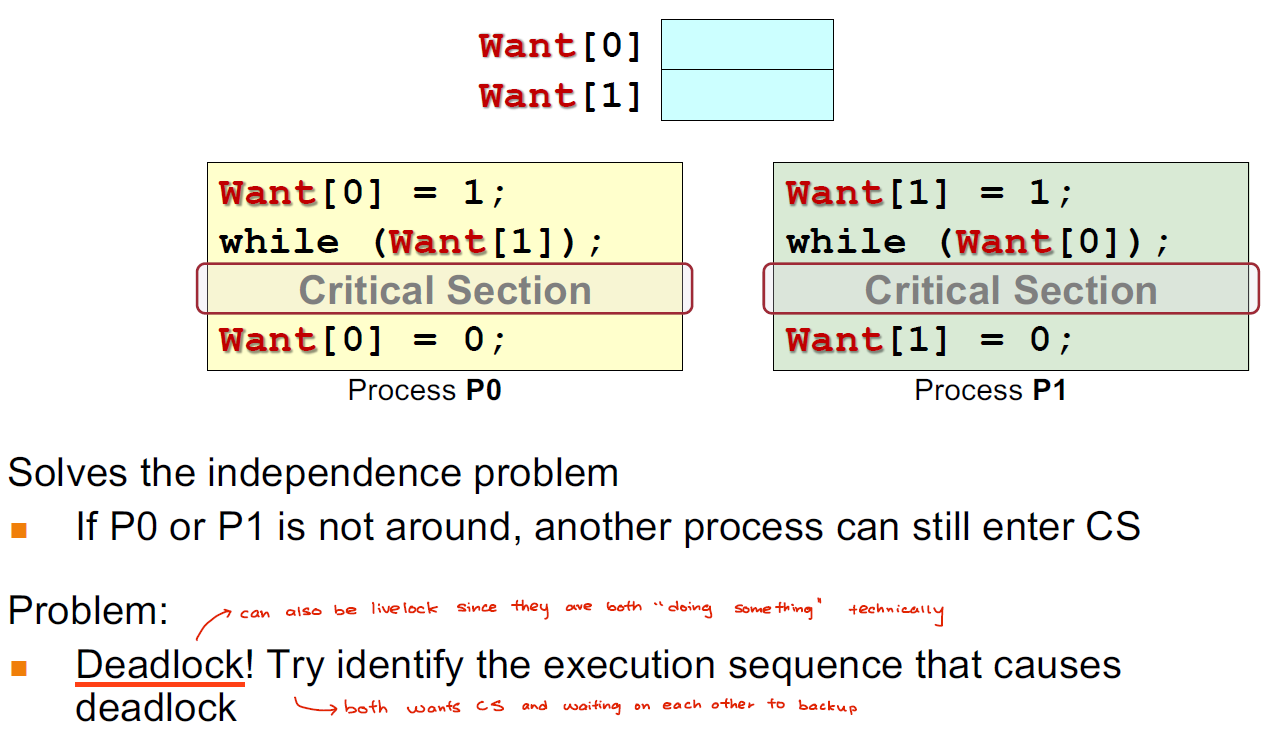
\includegraphics[width=0.9\columnwidth]{attempt_3}
        \end{center}
        \subsubsection{Peterson's Algorithms}
        \begin{center}
            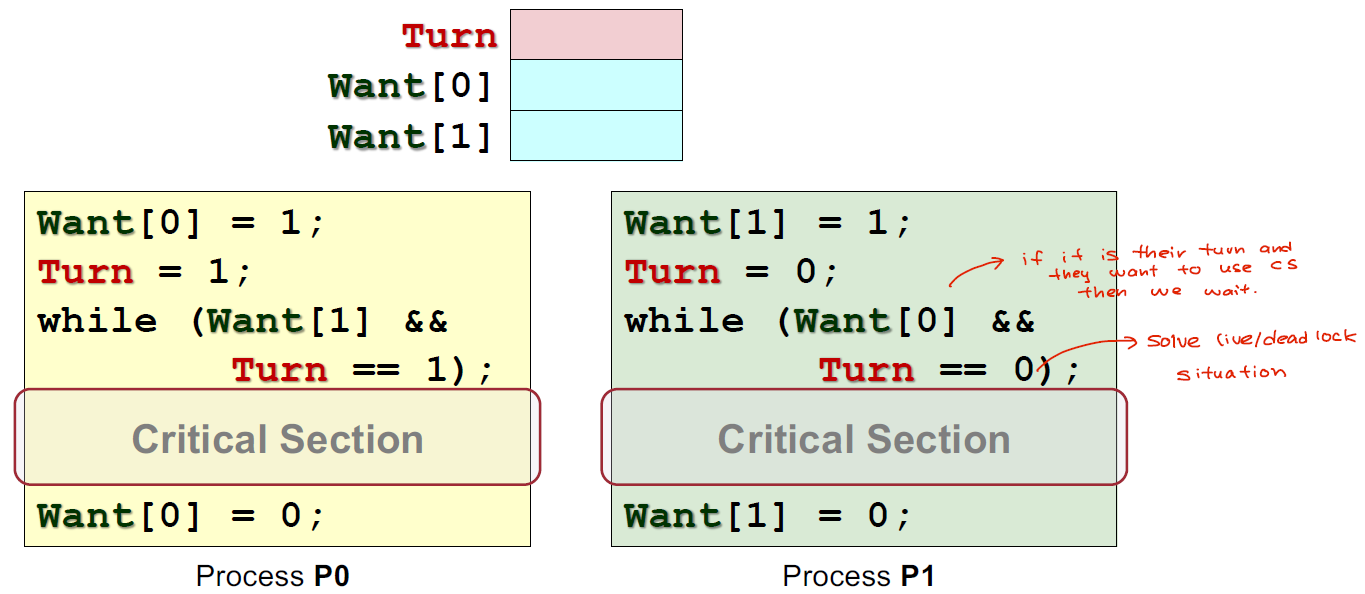
\includegraphics[width=0.9\columnwidth]{peterson}
        \end{center}
        * Note that the order of \texttt{Want[X] = 1} followed by \texttt{Turn = X} is important!
        \subsubsection{Peterson's Algorithm Disadvantages}
        \begin{itemize}
            \item \textbf{Busy Waiting}: wasteful use of processing power due to having while-loop instead of going into blocked state
            \item \textbf{Low level}: higher-level programming construct desirable to simplify mutex, make it less error prone and simpler to implement
            \item \textbf{Not general}: general synchronisation mechanism is desirable, not just mutex (limited to 2 processes)
        \end{itemize}
        \subsubsection{Test-and-set: an atomic instruction}
        \begin{itemize}
            \item Uses machine instructions to aid synchronization.
            \item Syntax: \texttt{TestAndSet Register, MemoryLocation}
            \item Load the current content at \texttt{MemoryLocation} into \texttt{Register}, Stores a \texttt{1} into \texttt{MemoryLocation}
            \item TestAndSet is performed as a single \textcolor{red}{atomic} machine operation and is \textbf{atomic even in multi-core system}
            \item Disadvantage: busy waiting (spin lock) -- wasteful use of processing power; Does not guarantee bounded-wait (unless scheduling is fair)
        \end{itemize}
        \subsubsection{Semaphore}
        A generalised synchronisation mechanism, providing a way to block a number of processes and a way to unblock one/more sleeping process(es)
        \begin{itemize}
            \item \texttt{wait(S)}: if $S > 0$, decrement. If $S \leq 0$, go to sleep
            \item \texttt{signal(S)}: increment $S$, wakes up one sleeping process (if any), operation \textcolor{red}{never blocks}
            \item done with the help of OS to ensure atomicity
            \item \textcolor{red}{no busy waiting} (processes are blocked while waiting)
            \item solves all known synchronization problems
        \end{itemize}
        \textbf{Properties}
        \begin{itemize}
            \item Given $S_\text{initial} \geq 0$, where \#signal(S) = number of \texttt{signal()} executed, \#wait(S) = number of \texttt{wait()} completed (successfully decremented $S$)
            \item \textbf{Invariant}: $S_{\texttt{current}} = S_{\texttt{Initial}} +$ \#signal($S$) $-$ \#wait($S$)
        \end{itemize}
        \subsubsection{Types of Semaphores}
        \begin{itemize}
            \item General Semaphores (Counting Semaphores): \textcolor{red}{$S \geq 0$}, useful for safe-distancing problem (limit number of processes running)
            \item Binary Semaphore (mutex): \textcolor{red}{$S = 0$ or $1$}, used to create mutual exclusion zone (critical section), $S$ is upper bounded to 1 (if \texttt{signal()} called when value is 1 $\rightarrow$ undefined behaviour)
            \item General Semaphores can be mimicked by binary semaphores
        \end{itemize}
        \subsubsection{Incorrect use of semaphore}
        \begin{center}
            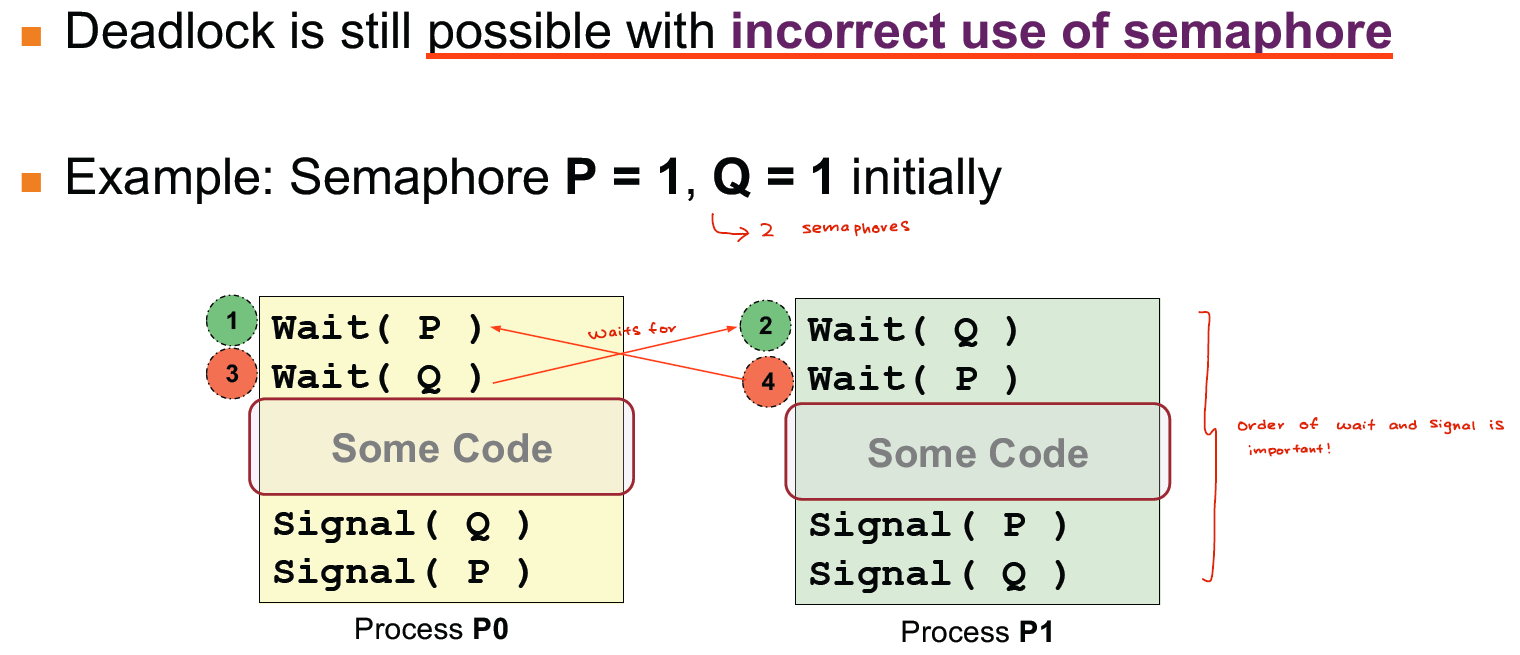
\includegraphics[width=0.8\columnwidth]{incorrect_semaphore}
        \end{center}
        %  Deadlock still possible
        %  \subsection{Classical Synchronisation Problems}
        %  \begin{itemize}
            %    \item \textbf{Producer-Consumer}: produce only if buffer not full, consume only if buffer not empty
            %    \item \textbf{Reader-Writers}: writer exclusive access, reader can share
            %    \item \textbf{Dining Philosophers}: assign partial order to the resources, establishing convention that all resources will be requested in order. E.g. label forks 1-5, and always pick up lower-numbered fork first.
            %  \end{itemize}
        %  \subsection{Synchronisation Implementations}
        %  \begin{itemize}
            %    \item POSIX semaphores
            %    \item pthread\_mutex\_t: \texttt{pthread\_mutex\_lock}, \texttt{pthread\_mutex\_unlock}
            %    \item pthread\_cond\_t: \texttt{pthread\_cond\_wait}, \texttt{pthread\_cond\_signal}, \texttt{pthread\_cond\_broadcast}
            %  \end{itemize}
        \section{Miscellaneous}
        \textbf{Process State Diagram}:
        \begin{center}
            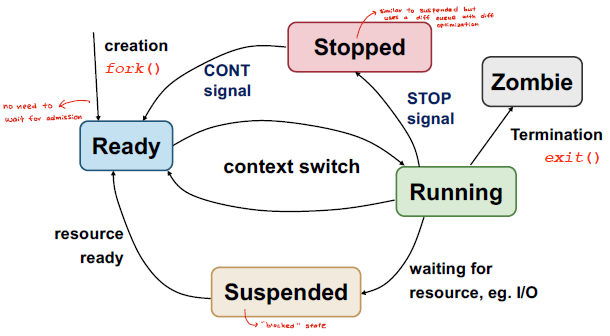
\includegraphics[width=0.7\columnwidth]{process-state-diagram}
        \end{center}
        \textbf{Priority Inversion}\\
        \begin{minipage}{\columnwidth}
            \makeatletter
            \newcommand{\@captype}{figure}
            \makeatother
            \centering
            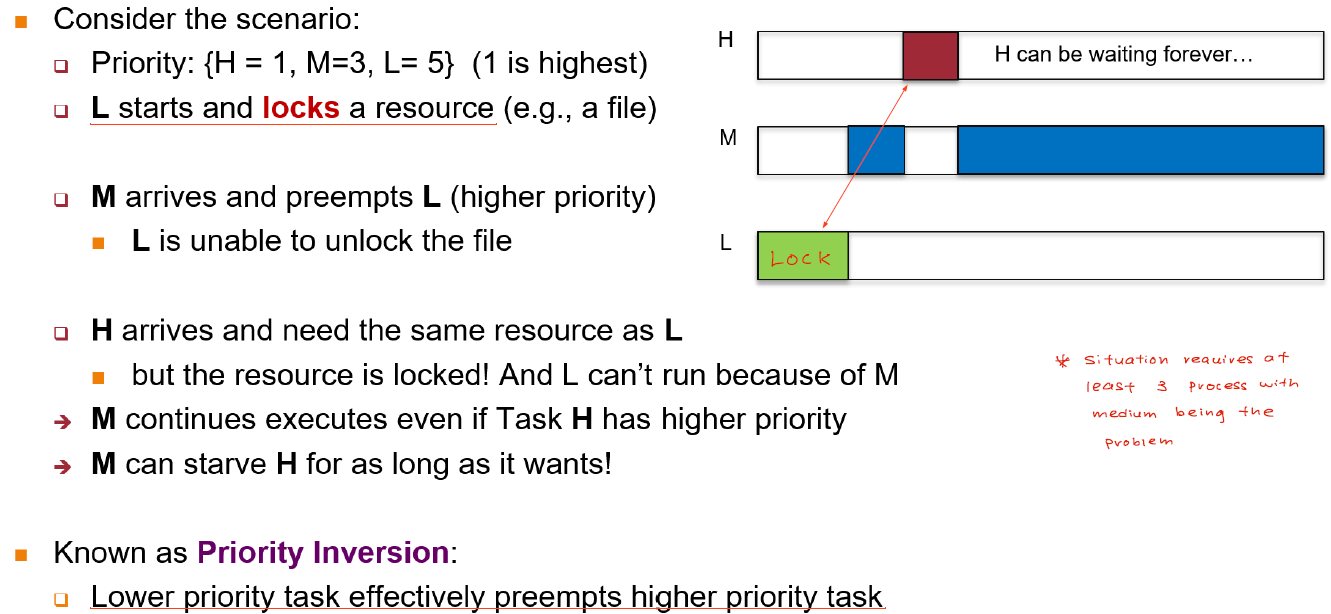
\includegraphics[width=0.7\columnwidth]{priority_inv}%
            \qquad%
            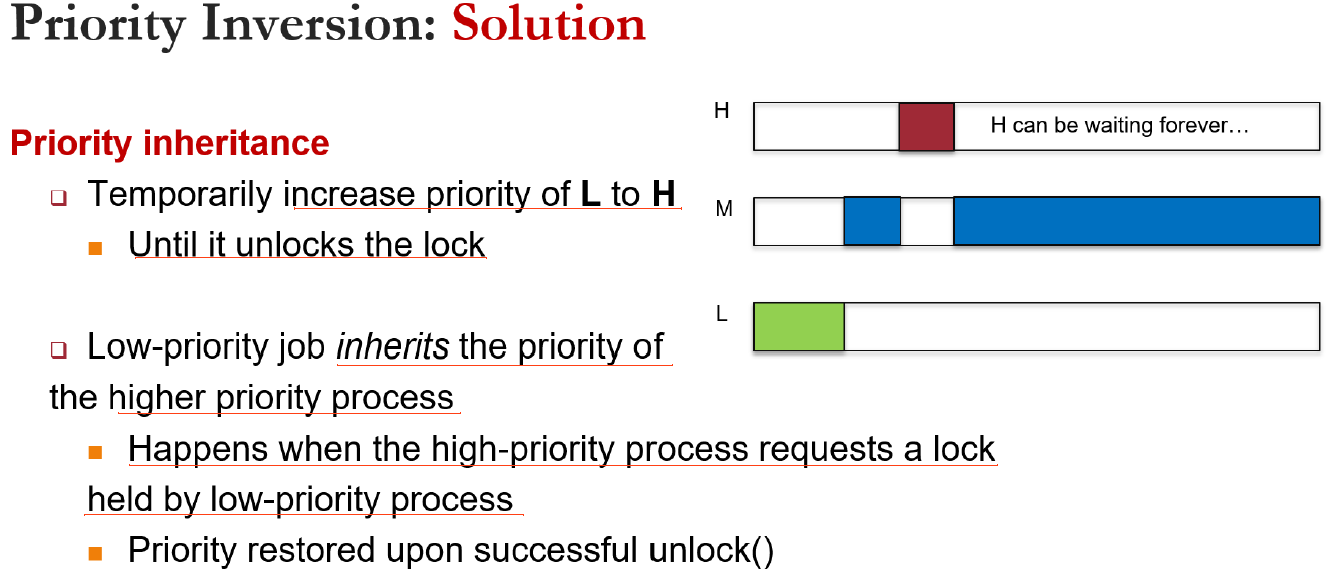
\includegraphics[width=0.7\columnwidth]{priority_inv_sol}%
        \end{minipage}
        \section{Office hours}
        \subsection{OS vs Kernel}
        \textbf{Kernel}:
        \begin{itemize}
            \item Essence of OS, manages and protects CPU, memory and other key resources
            \item doesn't use SYSCALLs, normal libraries and normal I/O
        \end{itemize}
        \textbf{OS}:
        \begin{itemize}
            \item Just a program with special features: deals with hardware issues, provides SYSCALLs, handles interrupts and device drivers
            \item User-friendly packaging of kernel: Includes lots of non-essential functionalities (GUI), superset of kernel
        \end{itemize}
        \subsection{Kernel mode}
        Kernel mode is the \textbf{most privileged mode of execution} in hardware which is mainly ran by the kernel. Other parts of OS use less privileged mode of execution.
        \subsubsection{Kernel mode vs Super user}
        \begin{itemize}
            \item Kernel mode is a mode of execution in hardware; when in this mode, you can execute any instruction with its fullest semantics. These privileges are reserved for the critical part of the kernel.
            \item Super-user privileges allow a certain user to manage users, files, and processes in an unrestricted manner. This removes certain OS-level restrictions, but not the hardware-level restrictions.
            \item Super user (e.g. \texttt{sudo}) $\neq$ kernel mode
        \end{itemize}
        \subsection{Return value}
        How does the return value gets accessed after the stackframe is torn down?
        \begin{itemize}
            \item \textcolor{red}{Teardown does NOT destroy anything!} Values from the function that returned still stays on stack frame until it is overwritten by other stack frames
            \item Teardown just changes the value of SP
        \end{itemize}

        \subsection{Stacks and Frames Exercise}
        \begin{center}
            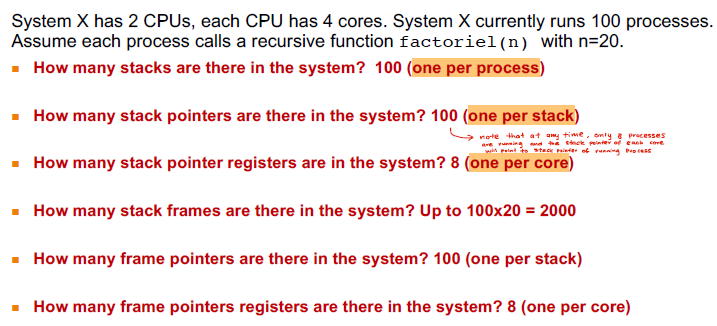
\includegraphics[width=0.8\columnwidth]{office_hours_exercise}
        \end{center}
        \subsection{Heap}
        Why dynamically allocated memory cannot use "Data" region?
        \begin{itemize}
            \item Size of data region is determined at compile time $\rightarrow$ fixed at runtime, dynamically allocated memory can be of any arbitrary size and is unknown at compile time
            \item Variables in data region lives for the duration of the program whereas dynamically allocated variables can live for as much time as the user wants (until user calls \texttt{free()})
        \end{itemize}
        \subsection{Interrupt Handling Steps}
        \begin{center}
            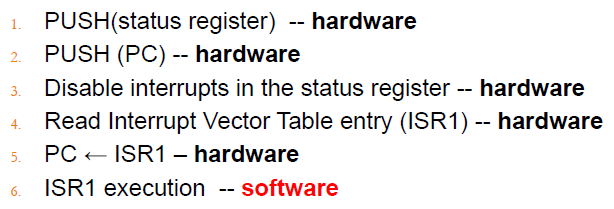
\includegraphics[width=0.8\columnwidth]{interrupt_handling}
            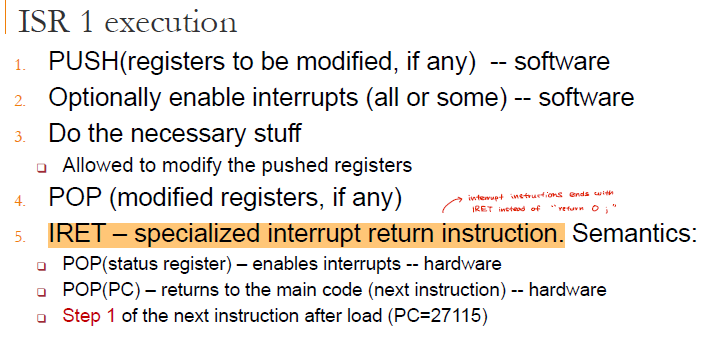
\includegraphics[width=0.8\columnwidth]{isr}
        \end{center}
        \vfill\null
        \columnbreak
        \subsection{Traps}
        Traps is an exception that is intentionally set-up (software-interrupt) and is used primarily as a means to enter kernel mode (e.g. for debugging purpose)
        \subsubsection{Traps vs Exceptions vs Traps}
        \begin{center}
            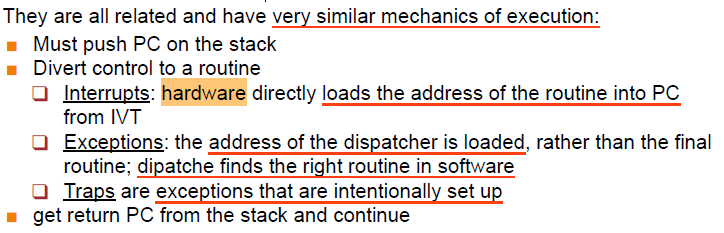
\includegraphics[width=0.8\columnwidth]{traps_exception_interrupts}
        \end{center}
        \subsection{How does fork bomb works}
        If a user runs: \mintinline{c}|while (1) { fork(); }|, it doesn't use any stack space so why would it cause problem?
        \begin{itemize}
            \item It is correct that this code does not use any stack space but since it is creating a new process and duplicating memory, there is some memory overhead (PCB, text, data, stack, heap etc.) which causes the system as a whole to run out of memory
        \end{itemize}
        \subsection{Preemptive vs Non-preemptive}
        \begin{itemize}
            \item Preemptive schedulers are needed to guarantee the responsiveness of the system
            \item Non-preemptive schedulers are used in simpler systems that do not care about responsiveness $\rightarrow$ overhead is lower
        \end{itemize}
        \subsection{Who schedule the scheduler?}
        \begin{itemize}
            \item Scheduler doesn't have to be scheduled
            \item In non-preemptive systems, when a process blocks/exits by calling a syscall, the scheduler is executed as well.
            \item For preemptive systems, the scheduler is called regularly by a timer interrupt.
        \end{itemize}
        \subsection{Scheduling Summary}
        \begin{center}
            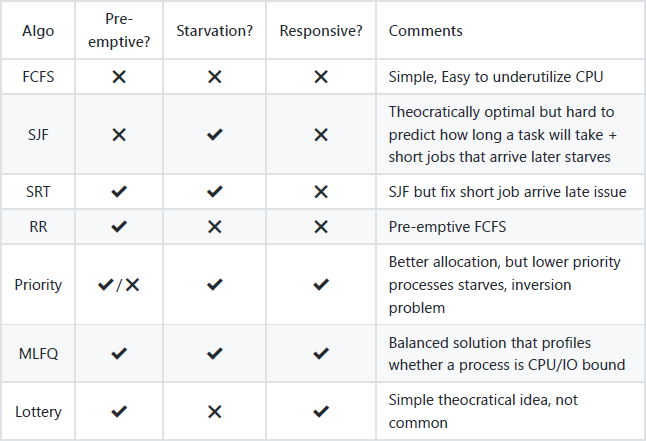
\includegraphics[width=0.7\columnwidth]{scheduling_summary}
        \end{center}
        \subsection{Are exceptions signals?}
        \begin{center}
            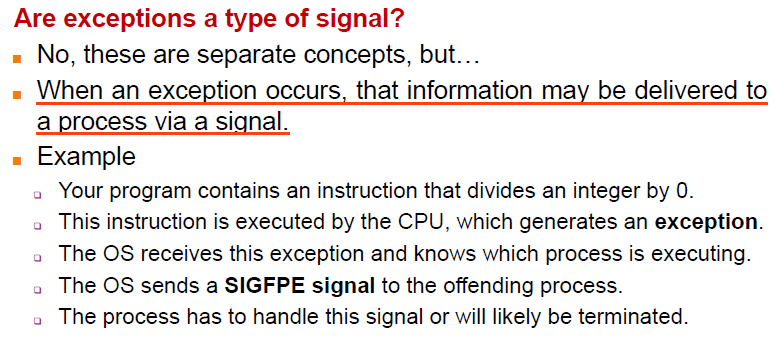
\includegraphics[width=0.7\columnwidth]{signal_exceptions}
        \end{center}
        \subsection{SRT Timer Interrupts?}
        \begin{center}
            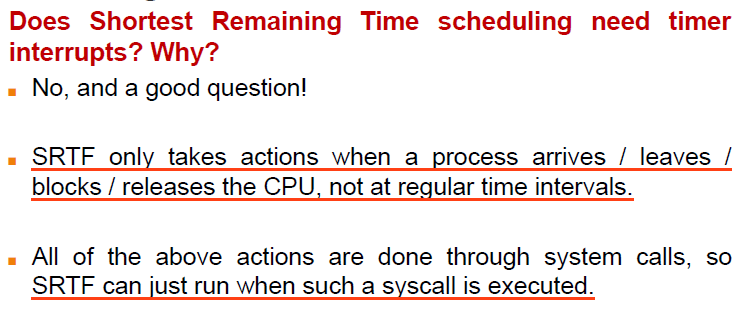
\includegraphics[width=0.7\columnwidth]{srt_timer}
        \end{center}
        \subsection{What makes lottery free of starvation?}
        \begin{center}
            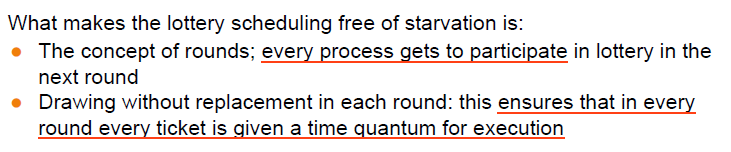
\includegraphics[width=0.9\columnwidth]{lottery_starvation_free}
        \end{center}
        \subsection{Indirect Message Passing}
        When do we use it?
        \begin{itemize}
            \item often used when it doesn't matter who
            received which message
            \item e.g. multiple clients send requests (messages) to a mailbox $\rightarrow$ mailbox buffers all the messages $\rightarrow$ multiple servers receive request from same mailbox
            \item No race conditions due to no shared data (data is copied from sender to buffer and buffer to reader) and also because OS takes care of integrity of its own message buffer
            \item Mailbox are cleaned up by the OS if process that created it crashes
        \end{itemize}
        \subsection{Kernel vs User space}
        \begin{center}
            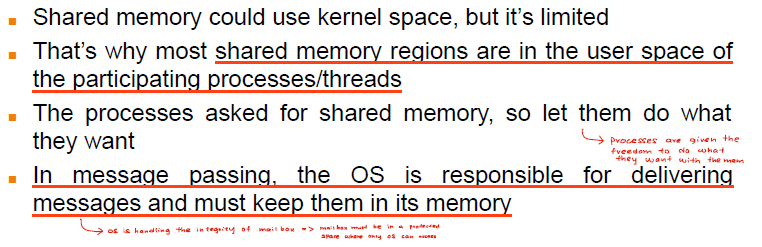
\includegraphics[width=0.9\columnwidth]{kernel_user_space}
        \end{center}
        \subsection{Kernel threads vs Actual processes}
        \begin{center}
            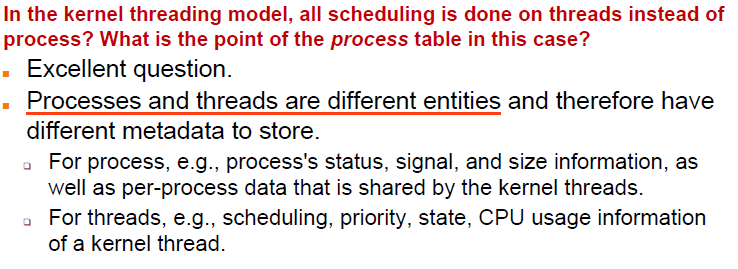
\includegraphics[width=0.9\columnwidth]{kernel_thread_vs_process}
        \end{center}
        \subsection{User thread stack}
        \begin{itemize}
            \item If OS not aware of user threads, where is the stack and register info stored?
            \item Program that manages the user thread must manage that information (likely to use heap memory to store)
            \item On top of memory management, these programs have to handle context switching, register spilling, reloading etc. on their own too
        \end{itemize}
        \subsection{Critical section properties}
        \begin{center}
            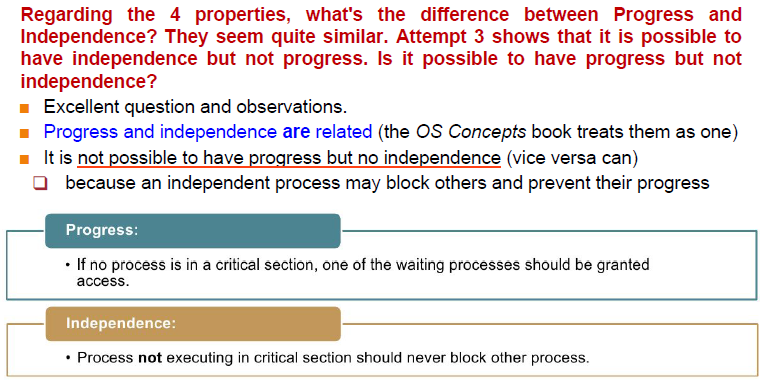
\includegraphics[width=0.9\columnwidth]{crit_section_prop}
        \end{center}
        \subsection{Uses of semaphores}
        \begin{enumerate}
            \item \textbf{Safe distancing problem}: allow only X number of processes to be running at the same time (General semaphore)
            \item \textbf{Mutex}: acts as a lock, no starvation under fair scheduling, no deadlock if used correctly, guarantees mutual exclusion (Binary semaphore)
            \item \textbf{Synchronization tool}: Execute B in \textit{$P_1$} only after A executed in \textit{$P_0$} (semaphore init to 0)
            \item \textbf{Barrier}: Only continue execution after all processes have reached barrier
        \end{enumerate}
        \end{multicols*}
\end{document}
